\documentclass{ximera}


\graphicspath{
  {./}
  {1-1QuantitativeReasoning/}
  {1-2RelationsAndGraphs/}
  {1-3ChangingInTandem/}
  {2-1LinearEquations/}
  {2-2LinearModeling/}
  {2-3ExponentialModeling/}
  {3-1WhatIsAFunction/}
  {3-2FunctionProperties/}
  {3-3AverageRatesOfChange/}
  {4-1BuildingNewFunctions/}
  {4-2Polynomials/}
  {5-1RationalFunctions/}
   {5-2ExponentialFunctions/}
  {6-1Domain/}
  {6-2Range/}
  {6-3CompositionOfFunctions/}
  {7-1ZerosOfFunctions/}
  {7-XZerosOfPolynomials/}
  {7-2ZerosOfFamousFunctions/}
  {8-0Review/}
  {8-1FunctionTransformations/}
  {8-2SolvingInequalities/}
  {8-3FunctionTransformationsProject/}
  {9-1RightTriangleTrig/}
  {9-2TheUnitCircle/}
  {9-3TrigIdentities/}
  {10-1UnitCircleToFunctionGraph/}
  {10-2TrigFunctions/}
  {10-3SomeApplicationsOfTrig/}
  {11-1InverseFunctionsRevisited/}
  {11-2Logarithms/}
  {11-3InverseTrig/}
  {12-1SystemsOfEquations/}
  {12-2NonlinearSystems/}
  {12-3ApplicationsOfSystems/}
  {13-1SecantLinesRevisited/}
  {13-2Functions-TheBigPicture/}
  {14-1DisplacementVsDistance/}
  {1-1QuantitativeReasoning/exercises/}
  {1-2RelationsAndGraphs/exercises/}
  {../1-3ChangingInTandem/exercises/}
  {../2-1LinearEquations/exercises/}
  {../2-2LinearModeling/exercises/}
  {../2-3ExponentialModeling/exercises/}
  {../3-1WhatIsAFunction/exercises/}
  {../3-2FunctionProperties/exercises/}
  {../3-3AverageRatesOfChange/exercises/}
  {../5-2ExponentialFunctions/exercises/}
  {../4-1BuildingNewFunctions/exercises/}
  {../4-2Polynomials/exercises/}
  {../5-1RationalFunctions/exercises/}
  {../6-1Domain/exercises/}
  {../6-2Range/exercises/}
  {../6-3CompositionOfFunctions/exercises/}
  {../7-1ZerosOfFunctions/exercises/}
  {../7-XZerosOfPolynomials/exercises/}
  {../7-2ZerosOfFamousFunctions/exercises/}
  {../8-1FunctionTransformations/exercises/}
  {../12-1SystemsOfEquations/exercises/}
  {../8-3FunctionTransformationsProject/exercises/}
  {../8-0Review/exercises/}
  {../8-2SolvingInequalities/exercises/}
  {../8-3FunctionTransformationsProject/exercises/}
  {../9-1RightTriangleTrig/exercises/}
  {../9-2TheUnitCircle/exercises/}
  {../9-3TrigIdentities/exercises/}
  {../10-1UnitCircleToFunctionGraph/exercises/}
  {../10-2TrigFunctions/exercises/}
  {../10-3SomeApplicationsOfTrig/exercises/}
  {../11-1InverseFunctionsRevisited/exercises/}
  {../11-2Logarithms/exercises/}
  {../11-3InverseTrig/exercises/}
  {../12-1SystemsOfEquations/exercises/}
  {../12-2NonlinearSystems/exercises/}
  {../12-3ApplicationsOfSystems/exercises/}
  {../13-1SecantLinesRevisited/exercises/}
  {../13-2Functions-TheBigPicture/exercises/}
  {../14-1DisplacementVsDistance/exercises/}
}

\DeclareGraphicsExtensions{.pdf,.png,.jpg,.eps}

\newcommand{\mooculus}{\textsf{\textbf{MOOC}\textnormal{\textsf{ULUS}}}}

\usepackage[makeroom]{cancel} %% for strike outs

\ifxake
\else
\usepackage[most]{tcolorbox}
\fi


%\typeout{************************************************}
%\typeout{New Environments}
%\typeout{************************************************}

%% to fix for web can be removed when deployed offically with ximera2
\let\image\relax\let\endimage\relax
\NewEnviron{image}{% 
  \begin{center}\BODY\end{center}% center
}



\NewEnviron{folder}{
      \addcontentsline{toc}{section}{\textbf{\BODY}}
}

\ifxake
\let\summary\relax
\let\endsummary\relax
\newtheorem*{summary}{Summary}
\newtheorem*{callout}{Callout}
\newtheorem*{overview}{Overview}
\newtheorem*{objectives}{Objectives}
\newtheorem*{motivatingQuestions}{Motivating Questions}
\newtheorem*{MM}{Metacognitive Moment}
      
%% NEEDED FOR XIMERA 2
%\ximerizedEnvironment{summary}
%\ximerizedEnvironment{callout}
%\ximerizedEnvironment{overview} 
%\ximerizedEnvironment{objectives}
%\ximerizedEnvironment{motivatingQuestions}
%\ximerizedEnvironment{MM}
\else
%% CALLOUT
\NewEnviron{callout}{
  \begin{tcolorbox}[colback=blue!5, breakable,pad at break*=1mm]
      \BODY
  \end{tcolorbox}
}
%% MOTIVATING QUESTIONS
\NewEnviron{motivatingQuestions}{
  \begin{tcolorbox}[ breakable,pad at break*=1mm]
    \textbf{\Large Motivating Questions}\hfill
    %\begin{itemize}[label=\textbullet]
      \BODY
    %\end{itemize}
  \end{tcolorbox}
}
%% OBJECTIVES
\NewEnviron{objectives}{  
    \vspace{.5in}
      %\begin{tcolorbox}[colback=orange!5, breakable,pad at break*=1mm]
    \textbf{\Large Learning Objectives}
    \begin{itemize}[label=\textbullet]
      \BODY
    \end{itemize}
    %\end{tcolorbox}
}
%% DEFINITION
\let\definition\relax
\let\enddefinition\relax
\NewEnviron{definition}{
  \begin{tcolorbox}[ breakable,pad at break*=1mm]
    \noindent\textbf{Definition}~
      \BODY
  \end{tcolorbox}
}
%% OVERVIEW
\let\overview\relax
\let\overview\relax
\NewEnviron{overview}{
  \begin{tcolorbox}[ breakable,pad at break*=1mm]
    \textbf{\Large Overview}
    %\begin{itemize}[label=\textbullet] %% breaks Xake
      \BODY
    %\end{itemize}
  \end{tcolorbox}
}
%% SUMMARY
\let\summary\relax
\let\endsummary\relax
\NewEnviron{summary}{
  \begin{tcolorbox}[ breakable,pad at break*=1mm]
    \textbf{\Large Summary}
    %\begin{itemize}[label=\textbullet] %% breaks Xake
      \BODY
    %\end{itemize}
  \end{tcolorbox}
}
%% REMARK
\let\remark\relax
\let\endremark\relax
\NewEnviron{remark}{
  \begin{tcolorbox}[colback=green!5, breakable,pad at break*=1mm]
    \noindent\textbf{Remark}~
      \BODY
  \end{tcolorbox}
}
%% EXPLANATION
\let\explanation\relax
\let\endexplanation\relax
\NewEnviron{explanation}{
    \normalfont
    \noindent\textbf{Explanation}~
      \BODY
}
%% EXPLORATION
\let\exploration\relax
\let\endexploration\relax
\NewEnviron{exploration}{
  \begin{tcolorbox}[colback=yellow!10, breakable,pad at break*=1mm]
    \noindent\textbf{Exploration}~
      \BODY
  \end{tcolorbox}
}
%% METACOGNITIVE MOMENTS
\let\MM\relax
\let\endMM\relax
\NewEnviron{MM}{
  \begin{tcolorbox}[colback=pink!15, breakable,pad at break*=1mm]
    \noindent\textbf{Metacognitive Moment}~
      \BODY
  \end{tcolorbox}
}


\fi





%Notes on what envirnoment to use:  Example with Explanation in text; if they are supposed to answer- Problem; no answer - Exploration


%\typeout{************************************************}
%% Header and footers
%\typeout{************************************************}

\newcommand{\licenseAcknowledgement}{Licensed under Creative Commons 4.0}
\newcommand{\licenseAPC}{\renewcommand{\licenseAcknowledgement}{\textbf{Acknowledgements:} Active Prelude to Calculus (https://activecalculus.org/prelude) }}
\newcommand{\licenseSZ}{\renewcommand{\licenseAcknowledgement}{\textbf{Acknowledgements:} Stitz Zeager Open Source Mathematics (https://www.stitz-zeager.com/) }}
\newcommand{\licenseAPCSZ}{\renewcommand{\licenseAcknowledgement}{\textbf{Acknowledgements:} Active Prelude to Calculus (https://activecalculus.org/prelude) and Stitz Zeager Open Source Mathematics (https://www.stitz-zeager.com/) }}
\newcommand{\licenseORCCA}{\renewcommand{\licenseAcknowledgement}{\textbf{Acknowledgements:}Original source material, products with readable and accessible
math content, and other information freely available at pcc.edu/orcca.}}
\newcommand{\licenseY}{\renewcommand{\licenseAcknowledgement}{\textbf{Acknowledgements:} Yoshiwara Books (https://yoshiwarabooks.org/)}}
\newcommand{\licenseOS}{\renewcommand{\licenseAcknowledgement}{\textbf{Acknowledgements:} OpenStax College Algebra (https://openstax.org/details/books/college-algebra)}}
\newcommand{\licenseAPCSZCSCC}{\renewcommand{\licenseAcknowledgement}{\textbf{Acknowledgements:} Active Prelude to Calculus (https://activecalculus.org/prelude), Stitz Zeager Open Source Mathematics (https://www.stitz-zeager.com/), CSCC PreCalculus and Calculus texts (https://ximera.osu.edu/csccmathematics)}}

\ifxake\else %% do nothing on the website
\usepackage{fancyhdr}
\pagestyle{fancy}
\fancyhf{}
\fancyhead[R]{\sectionmark}
\fancyfoot[L]{\thepage}
\fancyfoot[C]{\licenseAcknowledgement}
\renewcommand{\headrulewidth}{0pt}
\renewcommand{\footrulewidth}{0pt}
\fi

%%%%%%%%%%%%%%%%



%\typeout{************************************************}
%\typeout{Table of Contents}
%\typeout{************************************************}


%% Edit this to change the font style
\newcommand{\sectionHeadStyle}{\sffamily\bfseries}


\makeatletter

%% part uses arabic numerals
\renewcommand*\thepart{\arabic{part}}


\ifxake\else
\renewcommand\chapterstyle{%
  \def\maketitle{%
    \addtocounter{titlenumber}{1}%
    \pagestyle{fancy}
    \phantomsection
    \addcontentsline{toc}{section}{\textbf{\thepart.\thetitlenumber\hspace{1em}\@title}}%
                    {\flushleft\small\sectionHeadStyle\@pretitle\par\vspace{-1.5em}}%
                    {\flushleft\LARGE\sectionHeadStyle\thepart.\thetitlenumber\hspace{1em}\@title \par }%
                    {\setcounter{problem}{0}\setcounter{sectiontitlenumber}{0}}%
                    \par}}





\renewcommand\sectionstyle{%
  \def\maketitle{%
    \addtocounter{sectiontitlenumber}{1}
    \pagestyle{fancy}
    \phantomsection
    \addcontentsline{toc}{subsection}{\thepart.\thetitlenumber.\thesectiontitlenumber\hspace{1em}\@title}%
    {\flushleft\small\sectionHeadStyle\@pretitle\par\vspace{-1.5em}}%
    {\flushleft\Large\sectionHeadStyle\thepart.\thetitlenumber.\thesectiontitlenumber\hspace{1em}\@title \par}%
    %{\setcounter{subsectiontitlenumber}{0}}%
    \par}}



\renewcommand\section{\@startsection{paragraph}{10}{\z@}%
                                     {-3.25ex\@plus -1ex \@minus -.2ex}%
                                     {1.5ex \@plus .2ex}%
                                     {\normalfont\large\sectionHeadStyle}}
\renewcommand\subsection{\@startsection{subparagraph}{10}{\z@}%
                                    {3.25ex \@plus1ex \@minus.2ex}%
                                    {-1em}%
                                    {\normalfont\normalsize\sectionHeadStyle}}

\fi

%% redefine Part
\renewcommand\part{%
   {\setcounter{titlenumber}{0}}
  \if@openright
    \cleardoublepage
  \else
    \clearpage
  \fi
  \thispagestyle{plain}%
  \if@twocolumn
    \onecolumn
    \@tempswatrue
  \else
    \@tempswafalse
  \fi
  \null\vfil
  \secdef\@part\@spart}

\def\@part[#1]#2{%
    \ifnum \c@secnumdepth >-2\relax
      \refstepcounter{part}%
      \addcontentsline{toc}{part}{\thepart\hspace{1em}#1}%
    \else
      \addcontentsline{toc}{part}{#1}%
    \fi
    \markboth{}{}%
    {\centering
     \interlinepenalty \@M
     \normalfont
     \ifnum \c@secnumdepth >-2\relax
       \huge\sffamily\bfseries \partname\nobreakspace\thepart
       \par
       \vskip 20\p@
     \fi
     \Huge \bfseries #2\par}%
    \@endpart}
\def\@spart#1{%
    {\centering
     \interlinepenalty \@M
     \normalfont
     \Huge \bfseries #1\par}%
    \@endpart}
\def\@endpart{\vfil\newpage
              \if@twoside
               \if@openright
                \null
                \thispagestyle{empty}%
                \newpage
               \fi
              \fi
              \if@tempswa
                \twocolumn
                \fi}



\makeatother





%\typeout{************************************************}
%\typeout{Stuff from Ximera}
%\typeout{************************************************}



\usepackage{array}  %% This is for typesetting long division
\setlength{\extrarowheight}{+.1cm}
\newdimen\digitwidth
\settowidth\digitwidth{9}
\def\divrule#1#2{
\noalign{\moveright#1\digitwidth
\vbox{\hrule width#2\digitwidth}}}





\newcommand{\RR}{\mathbb R}
\newcommand{\R}{\mathbb R}
\newcommand{\N}{\mathbb N}
\newcommand{\Z}{\mathbb Z}

\newcommand{\sagemath}{\textsf{SageMath}}


\def\d{\,d}
%\renewcommand{\d}{\mathop{}\!d}
\newcommand{\dd}[2][]{\frac{\d #1}{\d #2}}
\newcommand{\pp}[2][]{\frac{\partial #1}{\partial #2}}
\renewcommand{\l}{\ell}
\newcommand{\ddx}{\frac{d}{\d x}}



%\newcommand{\unit}{\,\mathrm}
\newcommand{\unit}{\mathop{}\!\mathrm}
\newcommand{\eval}[1]{\bigg[ #1 \bigg]}
\newcommand{\seq}[1]{\left( #1 \right)}
\renewcommand{\epsilon}{\varepsilon}
\renewcommand{\phi}{\varphi}


\renewcommand{\iff}{\Leftrightarrow}

\DeclareMathOperator{\arccot}{arccot}
\DeclareMathOperator{\arcsec}{arcsec}
\DeclareMathOperator{\arccsc}{arccsc}
\DeclareMathOperator{\sign}{sign}


%\DeclareMathOperator{\divergence}{divergence}
%\DeclareMathOperator{\curl}[1]{\grad\cross #1}
\newcommand{\lto}{\mathop{\longrightarrow\,}\limits}

\renewcommand{\bar}{\overline}

\colorlet{textColor}{black}
\colorlet{background}{white}
\colorlet{penColor}{blue!50!black} % Color of a curve in a plot
\colorlet{penColor2}{red!50!black}% Color of a curve in a plot
\colorlet{penColor3}{red!50!blue} % Color of a curve in a plot
\colorlet{penColor4}{green!50!black} % Color of a curve in a plot
\colorlet{penColor5}{orange!80!black} % Color of a curve in a plot
\colorlet{penColor6}{yellow!70!black} % Color of a curve in a plot
\colorlet{fill1}{penColor!20} % Color of fill in a plot
\colorlet{fill2}{penColor2!20} % Color of fill in a plot
\colorlet{fillp}{fill1} % Color of positive area
\colorlet{filln}{penColor2!20} % Color of negative area
\colorlet{fill3}{penColor3!20} % Fill
\colorlet{fill4}{penColor4!20} % Fill
\colorlet{fill5}{penColor5!20} % Fill
\colorlet{gridColor}{gray!50} % Color of grid in a plot

\newcommand{\surfaceColor}{violet}
\newcommand{\surfaceColorTwo}{redyellow}
\newcommand{\sliceColor}{greenyellow}




\pgfmathdeclarefunction{gauss}{2}{% gives gaussian
  \pgfmathparse{1/(#2*sqrt(2*pi))*exp(-((x-#1)^2)/(2*#2^2))}%
}





%\typeout{************************************************}
%\typeout{ORCCA Preamble.Tex}
%\typeout{************************************************}


%% \usepackage{geometry}
%% \geometry{letterpaper,total={408pt,9.0in}}
%% Custom Page Layout Adjustments (use latex.geometry)
%% \usepackage{amsmath,amssymb}
%% \usepackage{pgfplots}
\usepackage{pifont}                                         %needed for symbols, s.a. airplane symbol
\usetikzlibrary{positioning,fit,backgrounds}                %needed for nested diagrams
\usetikzlibrary{calc,trees,positioning,arrows,fit,shapes}   %needed for set diagrams
\usetikzlibrary{decorations.text}                           %needed for text following a curve
\usetikzlibrary{arrows,arrows.meta}                         %needed for open/closed intervals
\usetikzlibrary{positioning,3d,shapes.geometric}            %needed for 3d number sets tower

%% NEEDED FOR XIMERA 1
%\usetkzobj{all}       %NO LONGER VALID
%%%%%%%%%%%%%%

\usepackage{tikz-3dplot}
\usepackage{tkz-euclide}                     %needed for triangle diagrams
\usepgfplotslibrary{fillbetween}                            %shade regions of a plot
\usetikzlibrary{shadows}                                    %function diagrams
\usetikzlibrary{positioning}                                %function diagrams
\usetikzlibrary{shapes}                                     %function diagrams
%%% global colors from https://www.pcc.edu/web-services/style-guide/basics/color/ %%%
\definecolor{ruby}{HTML}{9E0C0F}
\definecolor{turquoise}{HTML}{008099}
\definecolor{emerald}{HTML}{1c8464}
\definecolor{amber}{HTML}{c7502a}
\definecolor{amethyst}{HTML}{70485b}
\definecolor{sapphire}{HTML}{263c53}
\colorlet{firstcolor}{sapphire}
\colorlet{secondcolor}{turquoise}
\colorlet{thirdcolor}{emerald}
\colorlet{fourthcolor}{amber}
\colorlet{fifthcolor}{amethyst}
\colorlet{sixthcolor}{ruby}
\colorlet{highlightcolor}{green!50!black}
\colorlet{graphbackground}{white}
\colorlet{wood}{brown!60!white}
%%% curve, dot, and graph custom styles %%%
\pgfplotsset{firstcurve/.style      = {color=firstcolor,  mark=none, line width=1pt, {Kite}-{Kite}, solid}}
\pgfplotsset{secondcurve/.style     = {color=secondcolor, mark=none, line width=1pt, {Kite}-{Kite}, solid}}
\pgfplotsset{thirdcurve/.style      = {color=thirdcolor,  mark=none, line width=1pt, {Kite}-{Kite}, solid}}
\pgfplotsset{fourthcurve/.style     = {color=fourthcolor, mark=none, line width=1pt, {Kite}-{Kite}, solid}}
\pgfplotsset{fifthcurve/.style      = {color=fifthcolor,  mark=none, line width=1pt, {Kite}-{Kite}, solid}}
\pgfplotsset{highlightcurve/.style  = {color=highlightcolor,  mark=none, line width=5pt, -, opacity=0.3}}   % thick, opaque curve for highlighting
\pgfplotsset{asymptote/.style       = {color=gray, mark=none, line width=1pt, <->, dashed}}
\pgfplotsset{symmetryaxis/.style    = {color=gray, mark=none, line width=1pt, <->, dashed}}
\pgfplotsset{guideline/.style       = {color=gray, mark=none, line width=1pt, -}}
\tikzset{guideline/.style           = {color=gray, mark=none, line width=1pt, -}}
\pgfplotsset{altitude/.style        = {dashed, color=gray, thick, mark=none, -}}
\tikzset{altitude/.style            = {dashed, color=gray, thick, mark=none, -}}
\pgfplotsset{radius/.style          = {dashed, thick, mark=none, -}}
\tikzset{radius/.style              = {dashed, thick, mark=none, -}}
\pgfplotsset{rightangle/.style      = {color=gray, mark=none, -}}
\tikzset{rightangle/.style          = {color=gray, mark=none, -}}
\pgfplotsset{closedboundary/.style  = {color=black, mark=none, line width=1pt, {Kite}-{Kite},solid}}
\tikzset{closedboundary/.style      = {color=black, mark=none, line width=1pt, {Kite}-{Kite},solid}}
\pgfplotsset{openboundary/.style    = {color=black, mark=none, line width=1pt, {Kite}-{Kite},dashed}}
\tikzset{openboundary/.style        = {color=black, mark=none, line width=1pt, {Kite}-{Kite},dashed}}
\tikzset{verticallinetest/.style    = {color=gray, mark=none, line width=1pt, <->,dashed}}
\pgfplotsset{soliddot/.style        = {color=firstcolor,  mark=*, only marks}}
\pgfplotsset{hollowdot/.style       = {color=firstcolor,  mark=*, only marks, fill=graphbackground}}
\pgfplotsset{blankgraph/.style      = {xmin=-10, xmax=10,
                                        ymin=-10, ymax=10,
                                        axis line style={-, draw opacity=0 },
                                        axis lines=box,
                                        major tick length=0mm,
                                        xtick={-10,-9,...,10},
                                        ytick={-10,-9,...,10},
                                        grid=major,
                                        grid style={solid,gray!20},
                                        xticklabels={,,},
                                        yticklabels={,,},
                                        minor xtick=,
                                        minor ytick=,
                                        xlabel={},ylabel={},
                                        width=0.75\textwidth,
                                      }
            }
\pgfplotsset{numberline/.style      = {xmin=-10,xmax=10,
                                        minor xtick={-11,-10,...,11},
                                        xtick={-10,-5,...,10},
                                        every tick/.append style={thick},
                                        axis y line=none,
                                        y=15pt,
                                        axis lines=middle,
                                        enlarge x limits,
                                        grid=none,
                                        clip=false,
                                        axis background/.style={},
                                        after end axis/.code={
                                          \path (axis cs:0,0)
                                          node [anchor=north,yshift=-0.075cm] {\footnotesize 0};
                                        },
                                        every axis x label/.style={at={(current axis.right of origin)},anchor=north},
                                      }
            }
\pgfplotsset{openinterval/.style={color=firstcolor,mark=none,ultra thick,{Parenthesis}-{Parenthesis}}}
\pgfplotsset{openclosedinterval/.style={color=firstcolor,mark=none,ultra thick,{Parenthesis}-{Bracket}}}
\pgfplotsset{closedinterval/.style={color=firstcolor,mark=none,ultra thick,{Bracket}-{Bracket}}}
\pgfplotsset{closedopeninterval/.style={color=firstcolor,mark=none,ultra thick,{Bracket}-{Parenthesis}}}
\pgfplotsset{infiniteopeninterval/.style={color=firstcolor,mark=none,ultra thick,{Kite}-{Parenthesis}}}
\pgfplotsset{openinfiniteinterval/.style={color=firstcolor,mark=none,ultra thick,{Parenthesis}-{Kite}}}
\pgfplotsset{infiniteclosedinterval/.style={color=firstcolor,mark=none,ultra thick,{Kite}-{Bracket}}}
\pgfplotsset{closedinfiniteinterval/.style={color=firstcolor,mark=none,ultra thick,{Bracket}-{Kite}}}
\pgfplotsset{infiniteinterval/.style={color=firstcolor,mark=none,ultra thick,{Kite}-{Kite}}}
\pgfplotsset{interval/.style= {ultra thick, -}}
%%% cycle list of plot styles for graphs with multiple plots %%%
\pgfplotscreateplotcyclelist{pccstylelist}{%
  firstcurve\\%
  secondcurve\\%
  thirdcurve\\%
  fourthcurve\\%
  fifthcurve\\%
}
%%% default plot settings %%%
\pgfplotsset{every axis/.append style={
  axis x line=middle,    % put the x axis in the middle
  axis y line=middle,    % put the y axis in the middle
  axis line style={<->}, % arrows on the axis
  scaled ticks=false,
  tick label style={/pgf/number format/fixed},
  xlabel={$x$},          % default put x on x-axis
  ylabel={$y$},          % default put y on y-axis
  xmin = -7,xmax = 7,    % most graphs have this window
  ymin = -7,ymax = 7,    % most graphs have this window
  domain = -7:7,
  xtick = {-6,-4,...,6}, % label these ticks
  ytick = {-6,-4,...,6}, % label these ticks
  yticklabel style={inner sep=0.333ex},
  minor xtick = {-7,-6,...,7}, % include these ticks, some without label
  minor ytick = {-7,-6,...,7}, % include these ticks, some without label
  scale only axis,       % don't consider axis and tick labels for width and height calculation
  cycle list name=pccstylelist,
  tick label style={font=\footnotesize},
  legend cell align=left,
  grid = both,
  grid style = {solid,gray!20},
  axis background/.style={fill=graphbackground},
}}
\pgfplotsset{framed/.style={axis background/.style ={draw=gray}}}
%\pgfplotsset{framed/.style={axis background/.style ={draw=gray,fill=graphbackground,rounded corners=3ex}}}
%%% other tikz (not pgfplots) settings %%%
%\tikzset{axisnode/.style={font=\scriptsize,text=black}}
\tikzset{>=stealth}
%%% for nested diagram in types of numbers section %%%
\newcommand\drawnestedsets[4]{
  \def\position{#1}             % initial position
  \def\nbsets{#2}               % number of sets
  \def\listofnestedsets{#3}     % list of sets
  \def\reversedlistofcolors{#4} % reversed list of colors
  % position and draw labels of sets
  \coordinate (circle-0) at (#1);
  \coordinate (set-0) at (#1);
  \foreach \set [count=\c] in \listofnestedsets {
    \pgfmathtruncatemacro{\cminusone}{\c - 1}
    % label of current set (below previous nested set)
    \node[below=3pt of circle-\cminusone,inner sep=0]
    (set-\c) {\set};
    % current set (fit current label and previous set)
    \node[circle,inner sep=0,fit=(circle-\cminusone)(set-\c)]
    (circle-\c) {};
  }
  % draw and fill sets in reverse order
  \begin{scope}[on background layer]
    \foreach \col[count=\c] in \reversedlistofcolors {
      \pgfmathtruncatemacro{\invc}{\nbsets-\c}
      \pgfmathtruncatemacro{\invcplusone}{\invc+1}
      \node[circle,draw,fill=\col,inner sep=0,
      fit=(circle-\invc)(set-\invcplusone)] {};
    }
  \end{scope}
  }
\ifdefined\tikzset
\tikzset{ampersand replacement = \amp}
\fi
\newcommand{\abs}[1]{\left\lvert#1\right\rvert}
%\newcommand{\point}[2]{\left(#1,#2\right)}
\newcommand{\highlight}[1]{\definecolor{sapphire}{RGB}{59,90,125} {\color{sapphire}{{#1}}}}
\newcommand{\firsthighlight}[1]{\definecolor{sapphire}{RGB}{59,90,125} {\color{sapphire}{{#1}}}}
\newcommand{\secondhighlight}[1]{\definecolor{emerald}{RGB}{20,97,75} {\color{emerald}{{#1}}}}
\newcommand{\unhighlight}[1]{{\color{black}{{#1}}}}
\newcommand{\lowlight}[1]{{\color{lightgray}{#1}}}
\newcommand{\attention}[1]{\mathord{\overset{\downarrow}{#1}}}
\newcommand{\nextoperation}[1]{\mathord{\boxed{#1}}}
\newcommand{\substitute}[1]{{\color{blue}{{#1}}}}
\newcommand{\pinover}[2]{\overset{\overset{\mathrm{\ #2\ }}{|}}{\strut #1 \strut}}
\newcommand{\addright}[1]{{\color{blue}{{{}+#1}}}}
\newcommand{\addleft}[1]{{\color{blue}{{#1+{}}}}}
\newcommand{\subtractright}[1]{{\color{blue}{{{}-#1}}}}
\newcommand{\multiplyright}[2][\cdot]{{\color{blue}{{{}#1#2}}}}
\newcommand{\multiplyleft}[2][\cdot]{{\color{blue}{{#2#1{}}}}}
\newcommand{\divideunder}[2]{\frac{#1}{{\color{blue}{{#2}}}}}
\newcommand{\divideright}[1]{{\color{blue}{{{}\div#1}}}}
\newcommand{\negate}[1]{{\color{blue}{{-}}}\left(#1\right)}
\newcommand{\cancelhighlight}[1]{\definecolor{sapphire}{RGB}{59,90,125}{\color{sapphire}{{\cancel{#1}}}}}
\newcommand{\secondcancelhighlight}[1]{\definecolor{emerald}{RGB}{20,97,75}{\color{emerald}{{\bcancel{#1}}}}}
\newcommand{\thirdcancelhighlight}[1]{\definecolor{amethyst}{HTML}{70485b}{\color{amethyst}{{\xcancel{#1}}}}}
\newcommand{\lt}{<} %% Bart: WHY?
\newcommand{\gt}{>} %% Bart: WHY?
\newcommand{\amp}{&} %% Bart: WHY?


%%% These commands break Xake
%% \newcommand{\apple}{\text{🍎}}
%% \newcommand{\banana}{\text{🍌}}
%% \newcommand{\pear}{\text{🍐}}
%% \newcommand{\cat}{\text{🐱}}
%% \newcommand{\dog}{\text{🐶}}

\newcommand{\apple}{PICTURE OF APPLE}
\newcommand{\banana}{PICTURE OF BANANA}
\newcommand{\pear}{PICTURE OF PEAR}
\newcommand{\cat}{PICTURE OF CAT}
\newcommand{\dog}{PICTURE OF DOG}


%%%%% INDEX STUFF
\newcommand{\dfn}[1]{\textbf{#1}\index{#1}}
\usepackage{imakeidx}
\makeindex[intoc]
\makeatletter
\gdef\ttl@savemark{\sectionmark{}}
\makeatother












 % for drawing cube in Optimization problem
\usetikzlibrary{quotes,arrows.meta}
\tikzset{
  annotated cuboid/.pic={
    \tikzset{%
      every edge quotes/.append style={midway, auto},
      /cuboid/.cd,
      #1
    }
    \draw [every edge/.append style={pic actions, densely dashed, opacity=.5}, pic actions]
    (0,0,0) coordinate (o) -- ++(-\cubescale*\cubex,0,0) coordinate (a) -- ++(0,-\cubescale*\cubey,0) coordinate (b) edge coordinate [pos=1] (g) ++(0,0,-\cubescale*\cubez)  -- ++(\cubescale*\cubex,0,0) coordinate (c) -- cycle
    (o) -- ++(0,0,-\cubescale*\cubez) coordinate (d) -- ++(0,-\cubescale*\cubey,0) coordinate (e) edge (g) -- (c) -- cycle
    (o) -- (a) -- ++(0,0,-\cubescale*\cubez) coordinate (f) edge (g) -- (d) -- cycle;
    \path [every edge/.append style={pic actions, |-|}]
    (b) +(0,-5pt) coordinate (b1) edge ["x"'] (b1 -| c)
    (b) +(-5pt,0) coordinate (b2) edge ["y"] (b2 |- a)
    (c) +(3.5pt,-3.5pt) coordinate (c2) edge ["x"'] ([xshift=3.5pt,yshift=-3.5pt]e)
    ;
  },
  /cuboid/.search also={/tikz},
  /cuboid/.cd,
  width/.store in=\cubex,
  height/.store in=\cubey,
  depth/.store in=\cubez,
  units/.store in=\cubeunits,
  scale/.store in=\cubescale,
  width=10,
  height=10,
  depth=10,
  units=cm,
  scale=.1,
}

\author{Elizabeth Campolongo}
\licenseAPCSZ
%\license{Creative Commons Attribution-ShareAlike 4.0 International License}
%\acknowledgement{https://activecalculus.org/prelude/sec-trig-inverse.html, https://www.stitz-zeager.com/szprecalculus07042013.pdf}

\title{Other Inverse Trig Functions}

\begin{document}
\begin{abstract}
  
\end{abstract}
\maketitle


%\typeout{************************************************}
%\typeout{Motivating Questions}
%\typeout{************************************************}

\begin{motivatingQuestions}\begin{itemize}
%Often start a section. 
\item For the restricted sine, tangent, and secant functions, how do we define the corresponding arcsine, arctangent, and arcsecant functions?
\item What are the key properties of arcsine, arctangent, and arcsecant?
\end{itemize}\end{motivatingQuestions}


%\typeout{************************************************}
%\typeout{Introduction}
%\typeout{************************************************}



%\typeout{************************************************}
%\typeout{section}
%\typeout{************************************************}

\section{Introduction}
In the last section we defined {\it arccosine}, the inverse for cosine restricted to a single period. In this section we will explore the definition of similar inverse functions on restricted domains of sine, tangent, and secant. 

As we recalled last time,
\begin{itemize}
\item
A function $f$ has an inverse function if and only if there exists a function $g$ that undoes the work of $f$: that is, there is some function $g$, the inverse of $f$, for which $g(f(x)) = x$ for each $x$ in the domain of $f$, and $f(g(y)) = y$ for each $y$ in the range of $f$. 
%
\item A function $f$ has an inverse function if and only if the graph of $f$ passes the {\it Horizontal Line Test}.
%
\item When $f$ has an inverse, we know that ``$y = f(t)$'' and ``$t = f^{-1}(y)$'' are two different perspectives on the same statement.
\end{itemize}
%
\par
As with the cosine function, the trigonometric functions $f(t) = \sin(t)$, $h(t) = \tan(t)$, and $k(t) = \sec(t)$ are periodic, so they fail the horizontal line test. Hence, considering these functions on their full domains, neither has an inverse function. At the same time, it is reasonable to think about changing perspective and viewing angles as outputs in certain restricted settings, as we did with cosine. 


\section{The Arcsine Function}

We can develop an inverse function for a restricted version of the sine function in a similar way.  As with the cosine function, we need to choose an interval on which the sine function is always increasing or always decreasing in order to have the function pass the horizontal line test.  The standard choice is the domain $\Big[\!\!-\!\frac{\pi}{2}, \frac{\pi}{2}\Big]$ on which $f(t) = \sin(t)$ is increasing and attains all of the values in the range of the sine function.  Thus, we consider $f(t) = \sin(t)$ so that $f$ has domain $\Big[\!-\frac{\pi}{2}, \frac{\pi}{2}\Big]$ and range $\big[\!-1,1\big]$ and use this restricted function to define the corresponding arcsine function.%
\begin{definition}
Let $y = f(t) = \sin(t)$ be defined on the domain $\Big[\!\!-\!\frac{\pi}{2}, \frac{\pi}{2}\Big]$, and observe $f$ has the range $\big[\!-1,1\big]$.  For any real number $y$ that satisfies $-1 \leq y \leq 1$, the \dfn{arcsine of $\mathbf{y}$}, denoted%
\begin{equation*}
\arcsin(y)
\end{equation*}
is the angle $t$ satisfying $-\frac{\pi}{2} \leq t \leq \frac{\pi}{2}$ such that $\sin(t) = y$.
%
Note that we use $t=\sin^{-1}(y)$ interchangeably with with $t = \arcsin(y)$. 
\end{definition}

\begin{problem}
The goal of this activity is to understand key properties of the arcsine function in a way similar to our discussion of the arccosine function in the previous section. We will use our deductive reasoning skills a la Sherlock Holmes to build off our discussion from the last section.%
\begin{enumerate}
\item
Using the definition of arcsine given above, what are the domain and range of the arcsine function? \\
\begin{itemize}
\item The domain of arcsine is $[\answer{-1} , \answer{1}]$.
%
\item The range of arcsine is $\Big[\answer{-\frac{\pi}{2}},\answer{\frac{\pi}{2}}\Big]$.
\end{itemize}
%
\item Determine the following values exactly: 
\begin{itemize}
\item $\arcsin(-1) = \answer{-\frac{\pi}{2}}$ 
%
\item $\arcsin\Big(\!\!-\frac{\sqrt{2}}{2}\Big) = \answer{-\frac{\pi}{4}}$
%
\item $\arcsin(0) = \answer{0}$
%
\item $\arcsin\Big(\frac{1}{2}\Big) = \answer{\frac{\pi}{6}}$
%
\item $\arcsin\Big(\frac{\sqrt{3}}{2}\Big) = \answer{\frac{\pi}{3}}$
\end{itemize}
%
\item
On the axes provided below, sketch a careful plot of the restricted sine function on the interval $\Big[\!\!-\!\frac{\pi}{2},\frac{\pi}{2}\Big]$ along with its corresponding inverse, the arcsine function.  Label at least three points on each curve so that each point on the sine graph corresponds to a point on the arcsine graph.  In addition, sketch the line $y = t$ to demonstrate how the graphs are reflections of one another across this line.
%
%
\item True or false: $\arcsin(\sin(5\pi)) = 5\pi$? \wordChoice{\choice{true}\choice[correct]{false}} \\
Write a complete sentence to explain your reasoning.%
\end{enumerate}
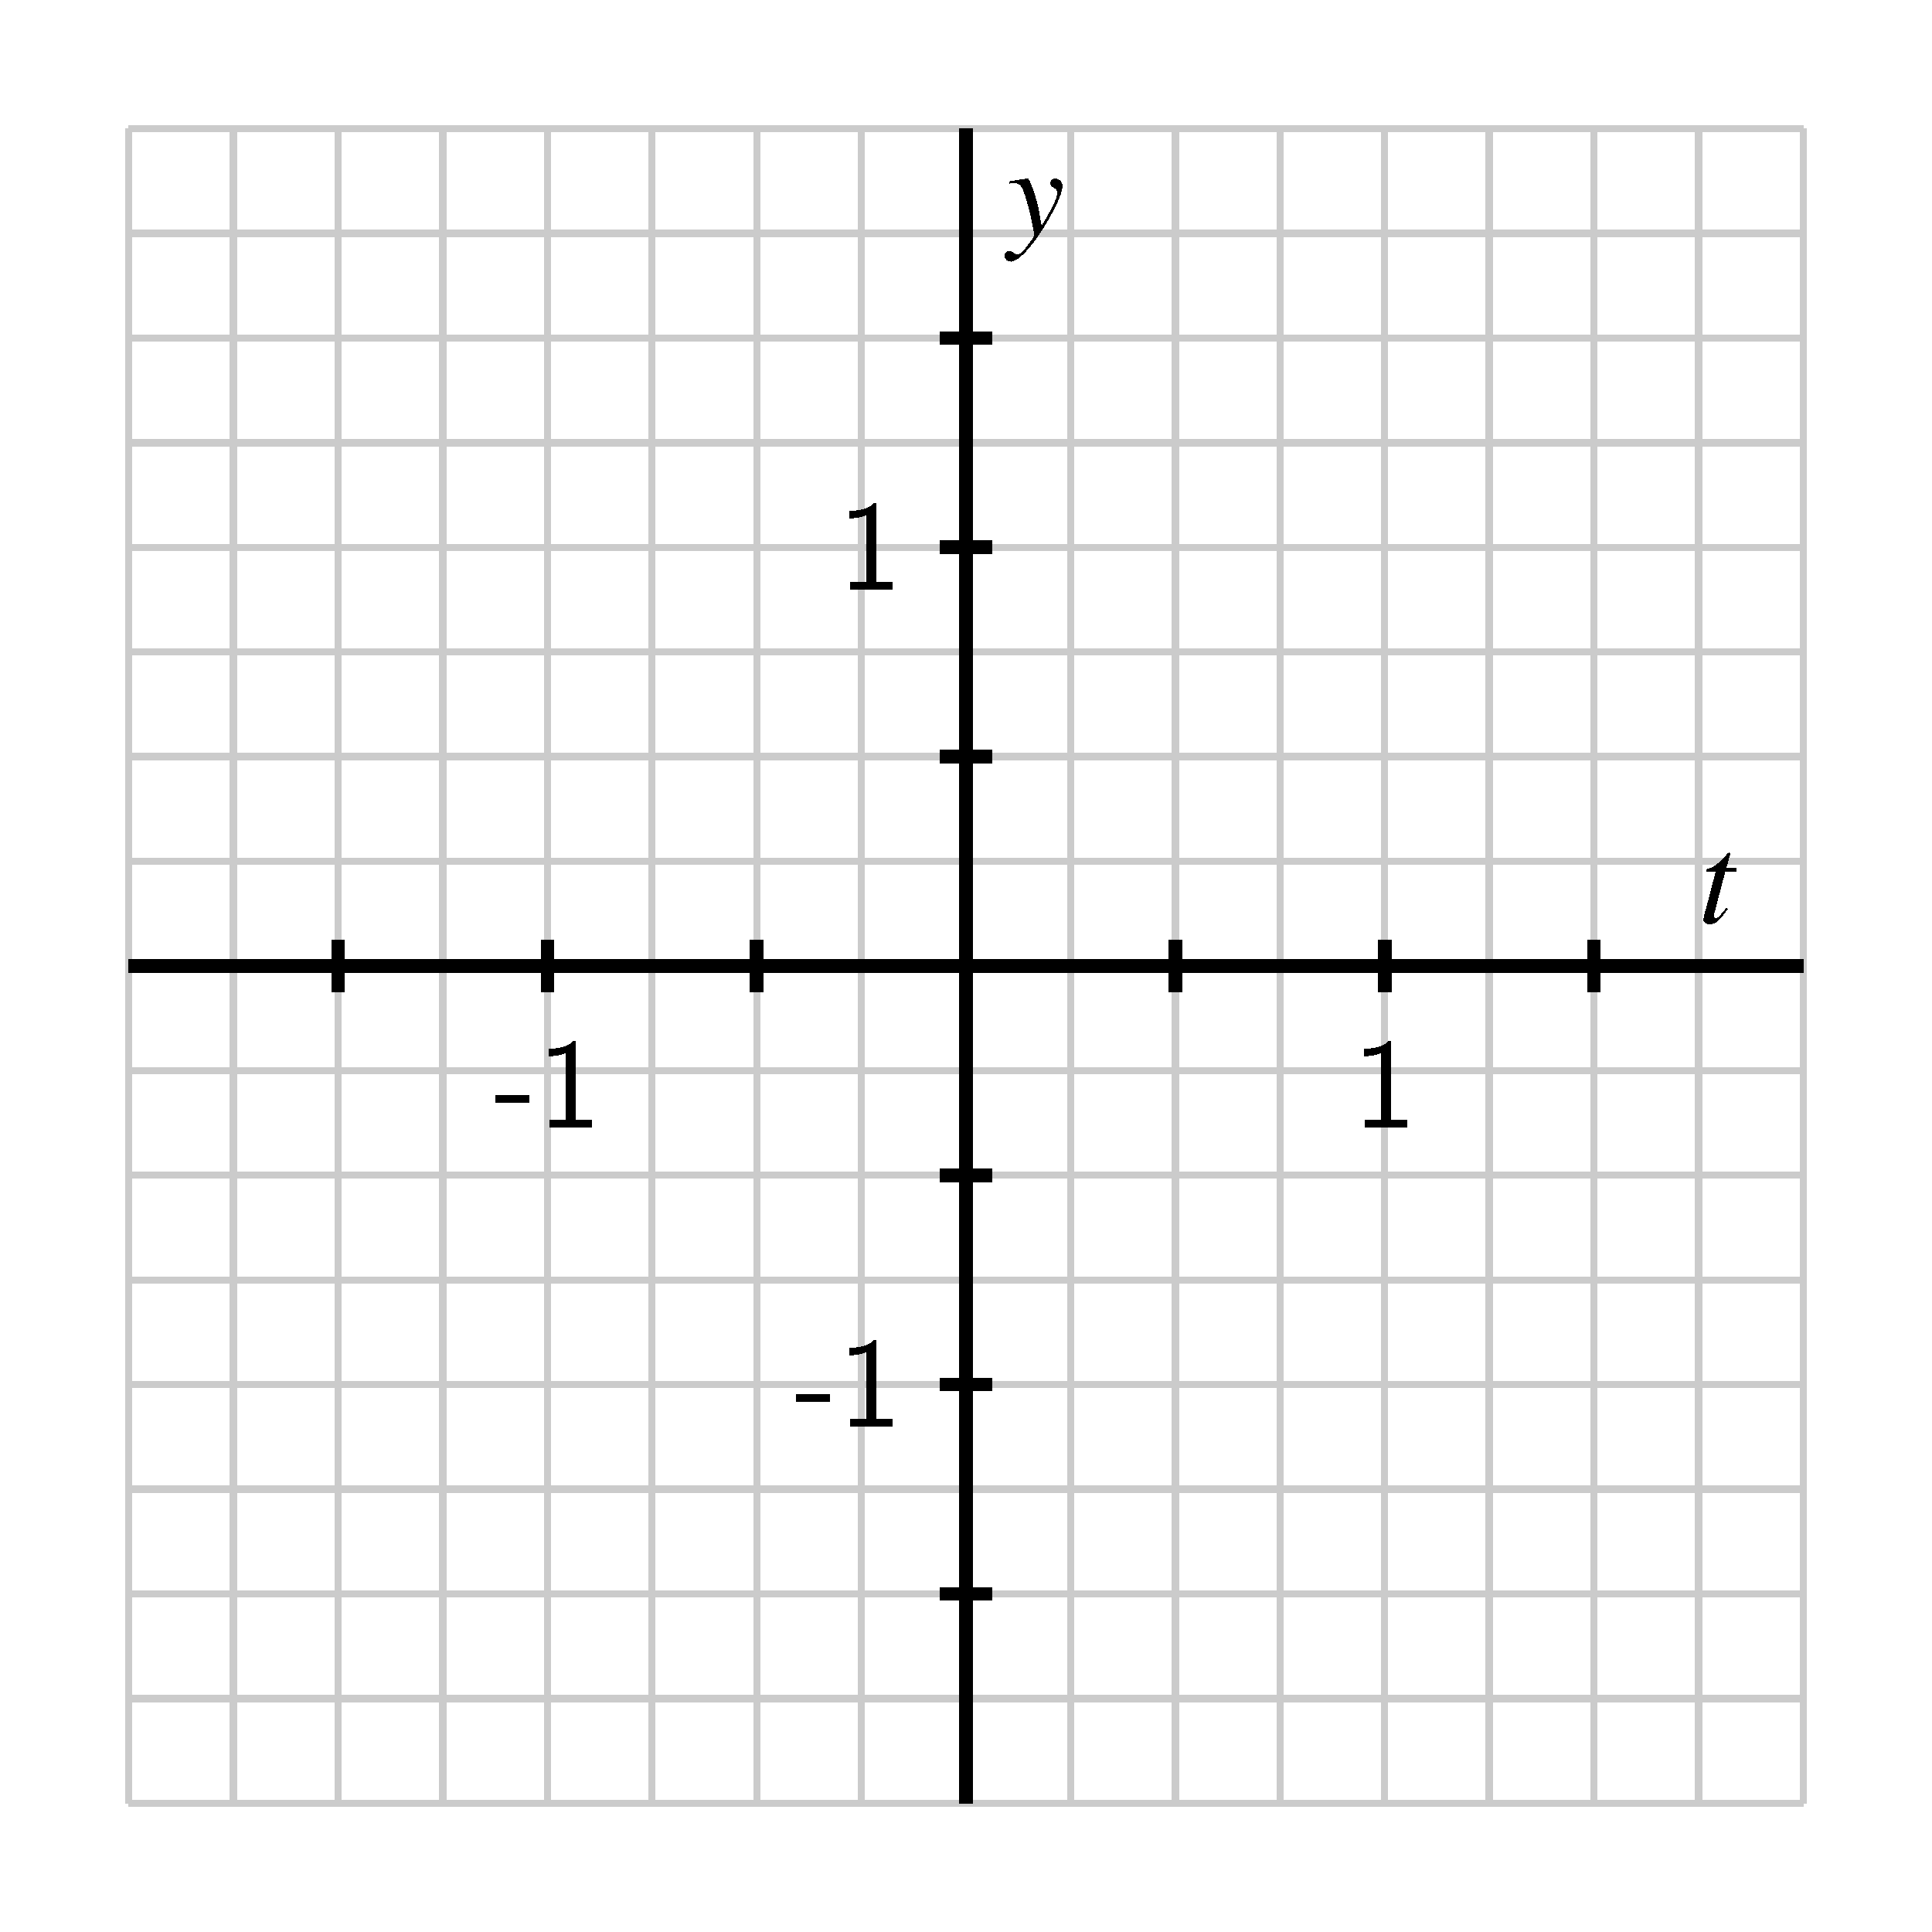
\includegraphics[width=1\linewidth]{inverse-trig-blank-axes-arcsin.png}
\end{problem}

\begin{callout}{\bf Properties of the arcsine function.}%
\begin{itemize}
\item
The restricted sine function, $y = f(t) = \sin(t)$, is defined on the domain $\Big[\!\!-\!\frac{\pi}{2},\frac{\pi}{2}\Big]$ with range $[-1,1]$.  This function has an inverse function that we call the arcsine function, denoted $t = f^{-1}(y) = \arcsin(y)$.%
\item
The domain of $y = f^{-1}(t) = \arcsin(t)$ is $[-1,1]$ with range $\Big[\!-\!\frac{\pi}{2},\frac{\pi}{2}\Big]$.%
\item
The arcsine function is always increasing on its domain.%
\item
Below we have a plot of the restricted sine function (in light blue) and its corresponding inverse, the arcsine function (in dark blue).%
\end{itemize}
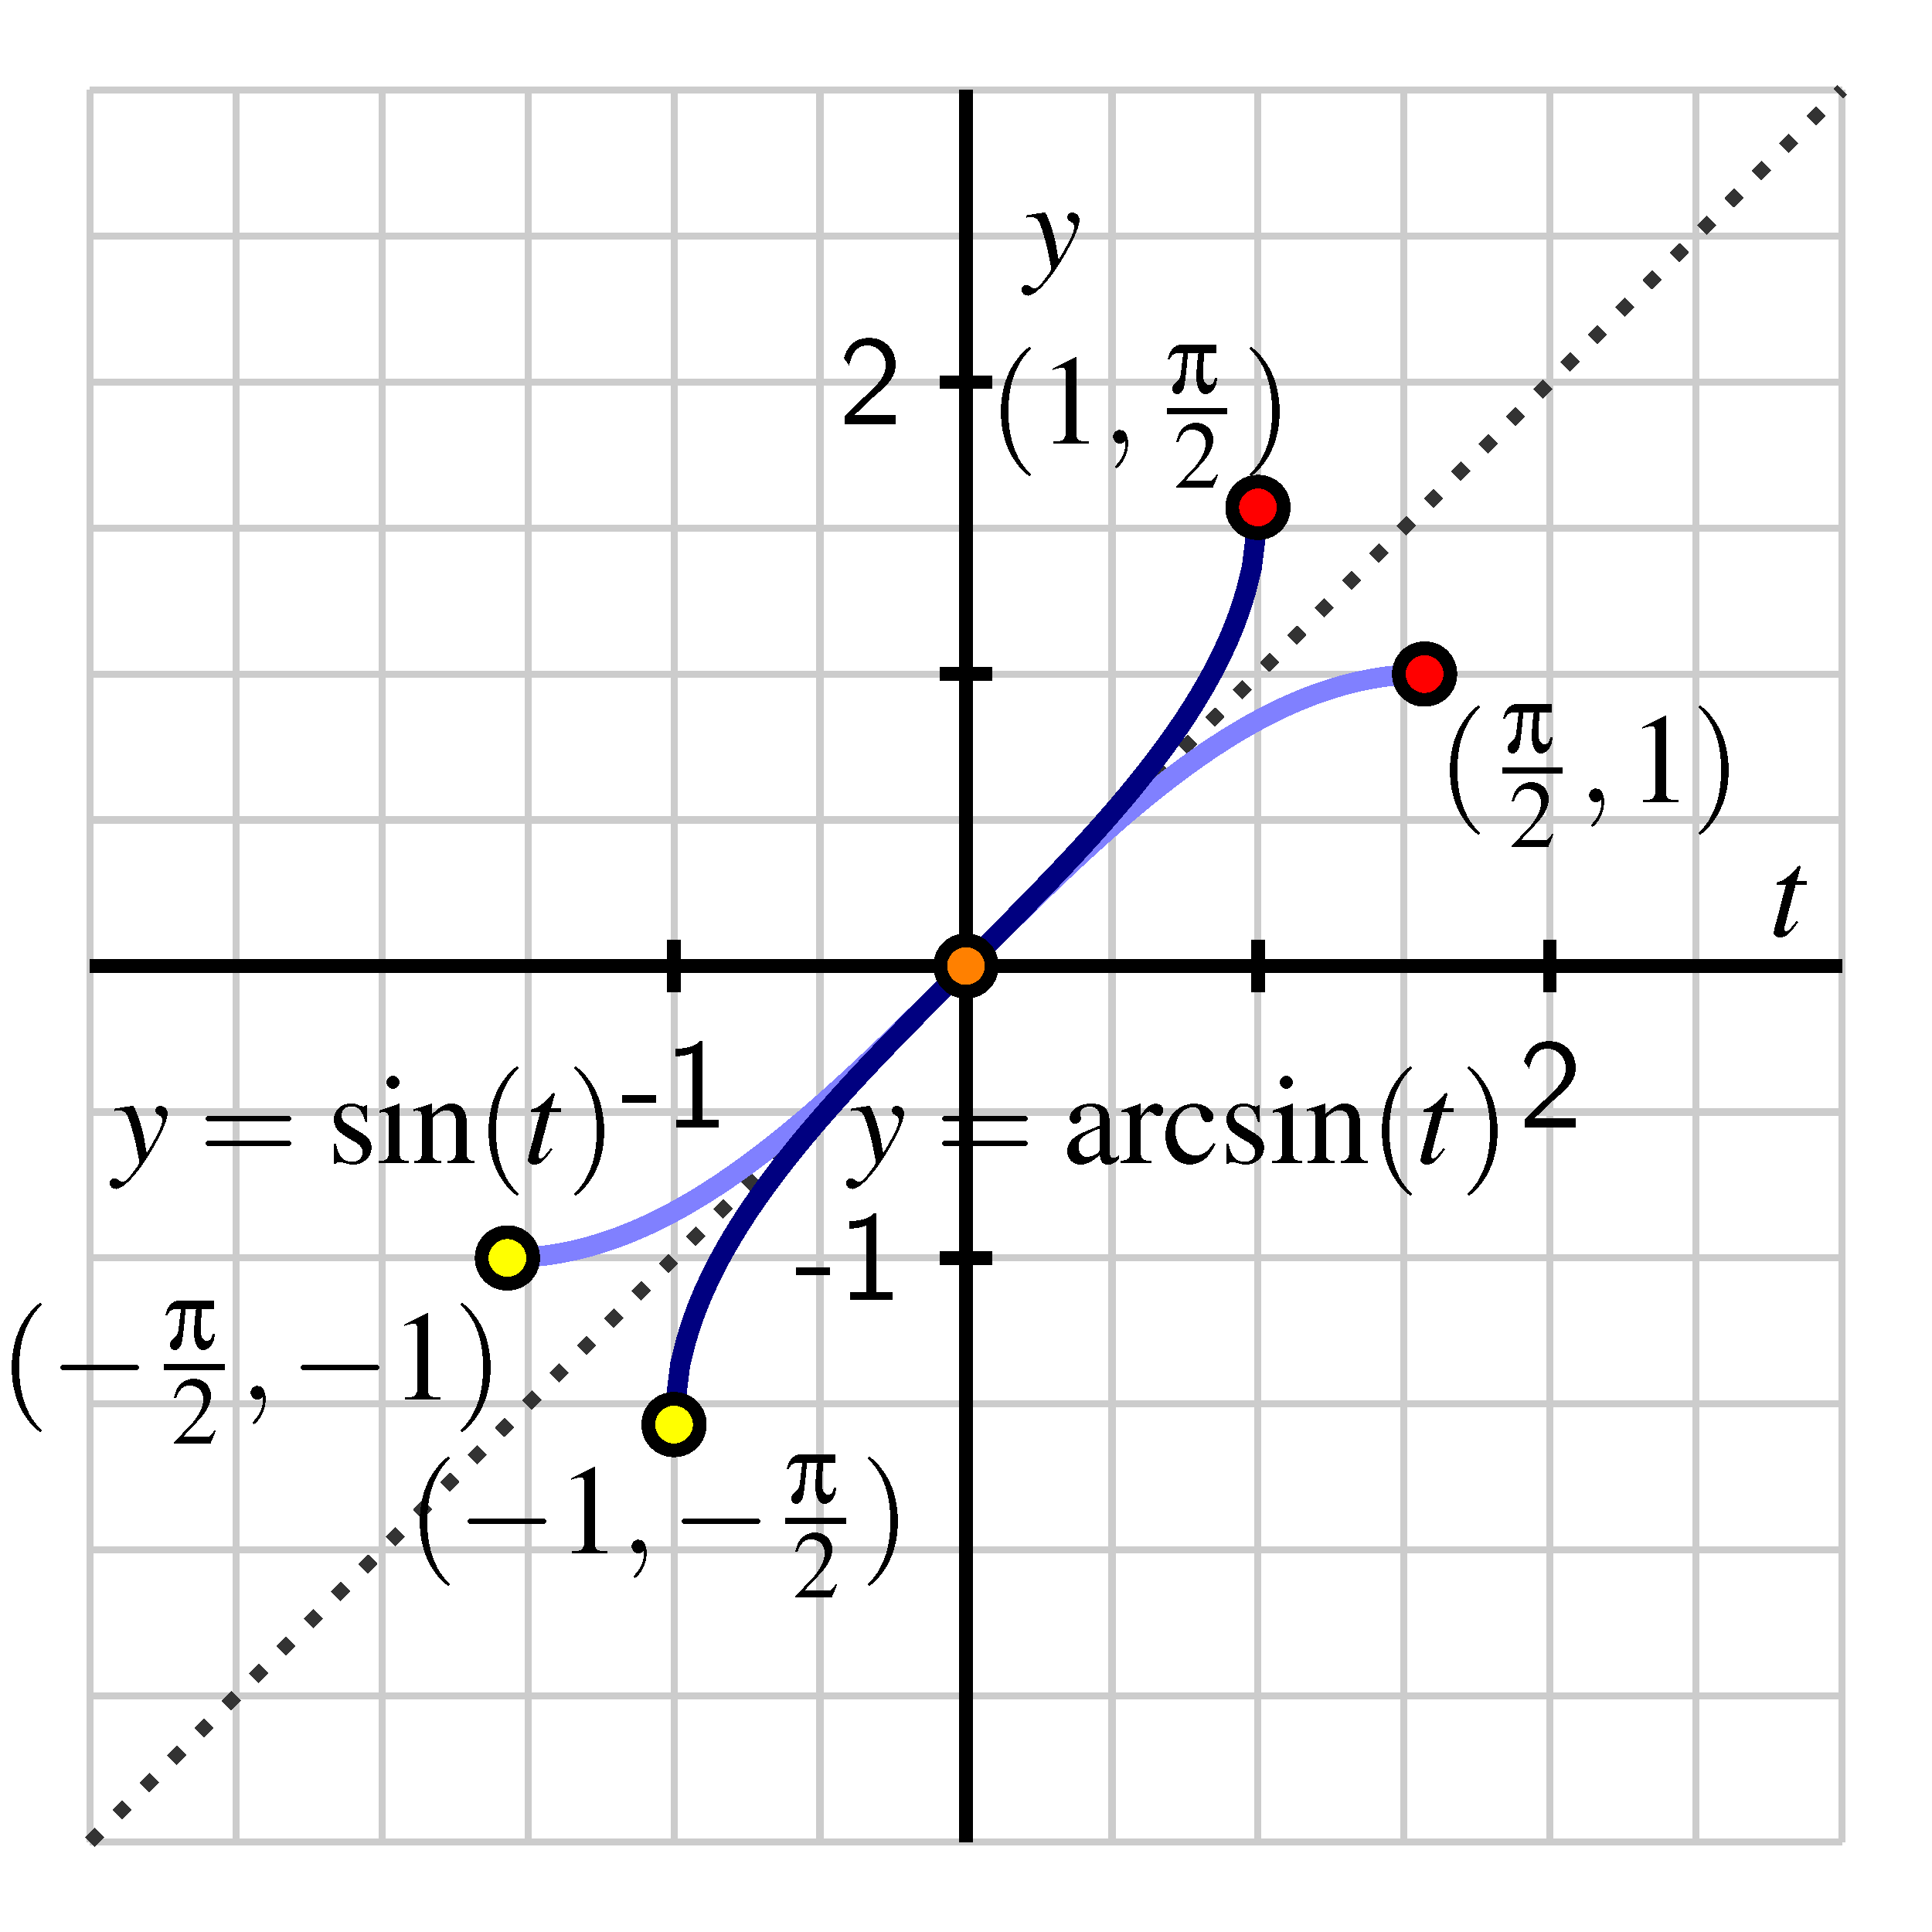
\includegraphics[width=1\linewidth]{inverse-trig-arcsin-graph.png}
\end{callout}

\section{Exploring Arcsine}

\begin{example}
Let's solve the following equations analytically, then we can consider the graph of arcsine.

\begin{enumerate}
\item $\sin\!\Big(\!\arcsin\!\Big(\!-\frac{\sqrt{2}}{2}\Big)\Big)$\\
\begin{explanation}
We start by finding $\arcsin\!\Big(\!\!-\!\frac{\sqrt{2}}{2}\Big)$. Remember that for $x$ in $[-1,1]$, $\arcsin(x)$ is the value $y$ in $\Big[-\frac{\pi}{2},\frac{\pi}{2}\Big]$ such that $\sin(y) = x$. 

Hence, $y$ is $-\frac{\pi}{4}$, and we now see that 
\begin{equation*}
\sin\!\Big(\!\arcsin\!\Big(\!\!-\!\frac{\sqrt{2}}{2}\Big)\Big) = \sin\Big(\!-\frac{\pi}{4}\Big) = -\frac{\sqrt{2}}{2}.
\end{equation*}

Now, if you're thinking, ``Hey, we didn't need that extra step!" Then you would be correct. But \textbf{\textit{why}} didn't we need that final step?

Let's recall how we defined arcsine. Since sine is a periodic function, it fails the horizontal line test. However, if we {\it restrict} sine to a portion of its domain on which it is only increasing, $\Big[-\frac{\pi}{2},\frac{\pi}{2}\Big]$, then we may define a function $f$ on this domain such that $f(x) = \sin(x)$ for $x$ in $\Big[-\frac{\pi}{2},\frac{\pi}{2}\Big]$. Arcsine then is defined as the inverse of this function $f$. Therefore, $f$ is the inverse of arcsine. 
Thus, in practice, sine is the inverse of arcsine. 

A word of caution: As was the case with arccosine and cosine, arcsine is only the inverse of restricted sine. We will illustrate this with the next example.
\end{explanation}


\item $\arcsin\!\Big(\sin\!\Big(\frac{5\pi}{4}\Big)\Big)$

\begin{explanation}
It may be tempting to take a look at this expression and conclude that the solution is $\frac{5\pi}{4}$ since arcsine is the inverse of sine. 

{\bf Hold those horses! }

Remember, we had to restrict the domain of sine in order to define an inverse function, which we called arcsine. Arcsine is the inverse of the {\it restricted} sine function, whose domain is $\Big[\!-\frac{\pi}{2},\frac{\pi}{2}\Big]$. $\frac{5\pi}{4}$ is larger than $\frac{\pi}{2}$, so it is not within the domain of this restricted sine function. 

Thus, we begin by simplifying $\sin\!\Big(\frac{5\pi}{4}\Big) = -\frac{\sqrt{2}}{2}$. 

Now, let's consider $\arcsin\!\Big(\!\!-\!\frac{\sqrt{2}}{2}\Big)$, recalling again the {\it range} of arcsine. We are looking for the value of $y$ in $\Big[\!-\frac{\pi}{2},\frac{\pi}{2}\Big]$ such that $\sin(y) =-\frac{\sqrt{2}}{2}$.

Hence, $y$ is $-\frac{\pi}{4}$, and we now see that 
\begin{equation*}
\arcsin\!\Big(\sin\!\Big(\frac{5\pi}{4}\Big)\Big) = \arcsin\!\Big(\!\!-\!\frac{\sqrt{2}}{2}\Big) = -\frac{\pi}{4}.
\end{equation*}

%Now, let's look again at the graph of cosine. Here we highlight $g: [0,\pi] \rightarrow [0,\pi]$ defined by $y=g(x)=\cos(x)$, the restricted cosine function. We may use the symmetry of the graph of cosine to help find the appropriate values for arccosine.
%\begin{image}
%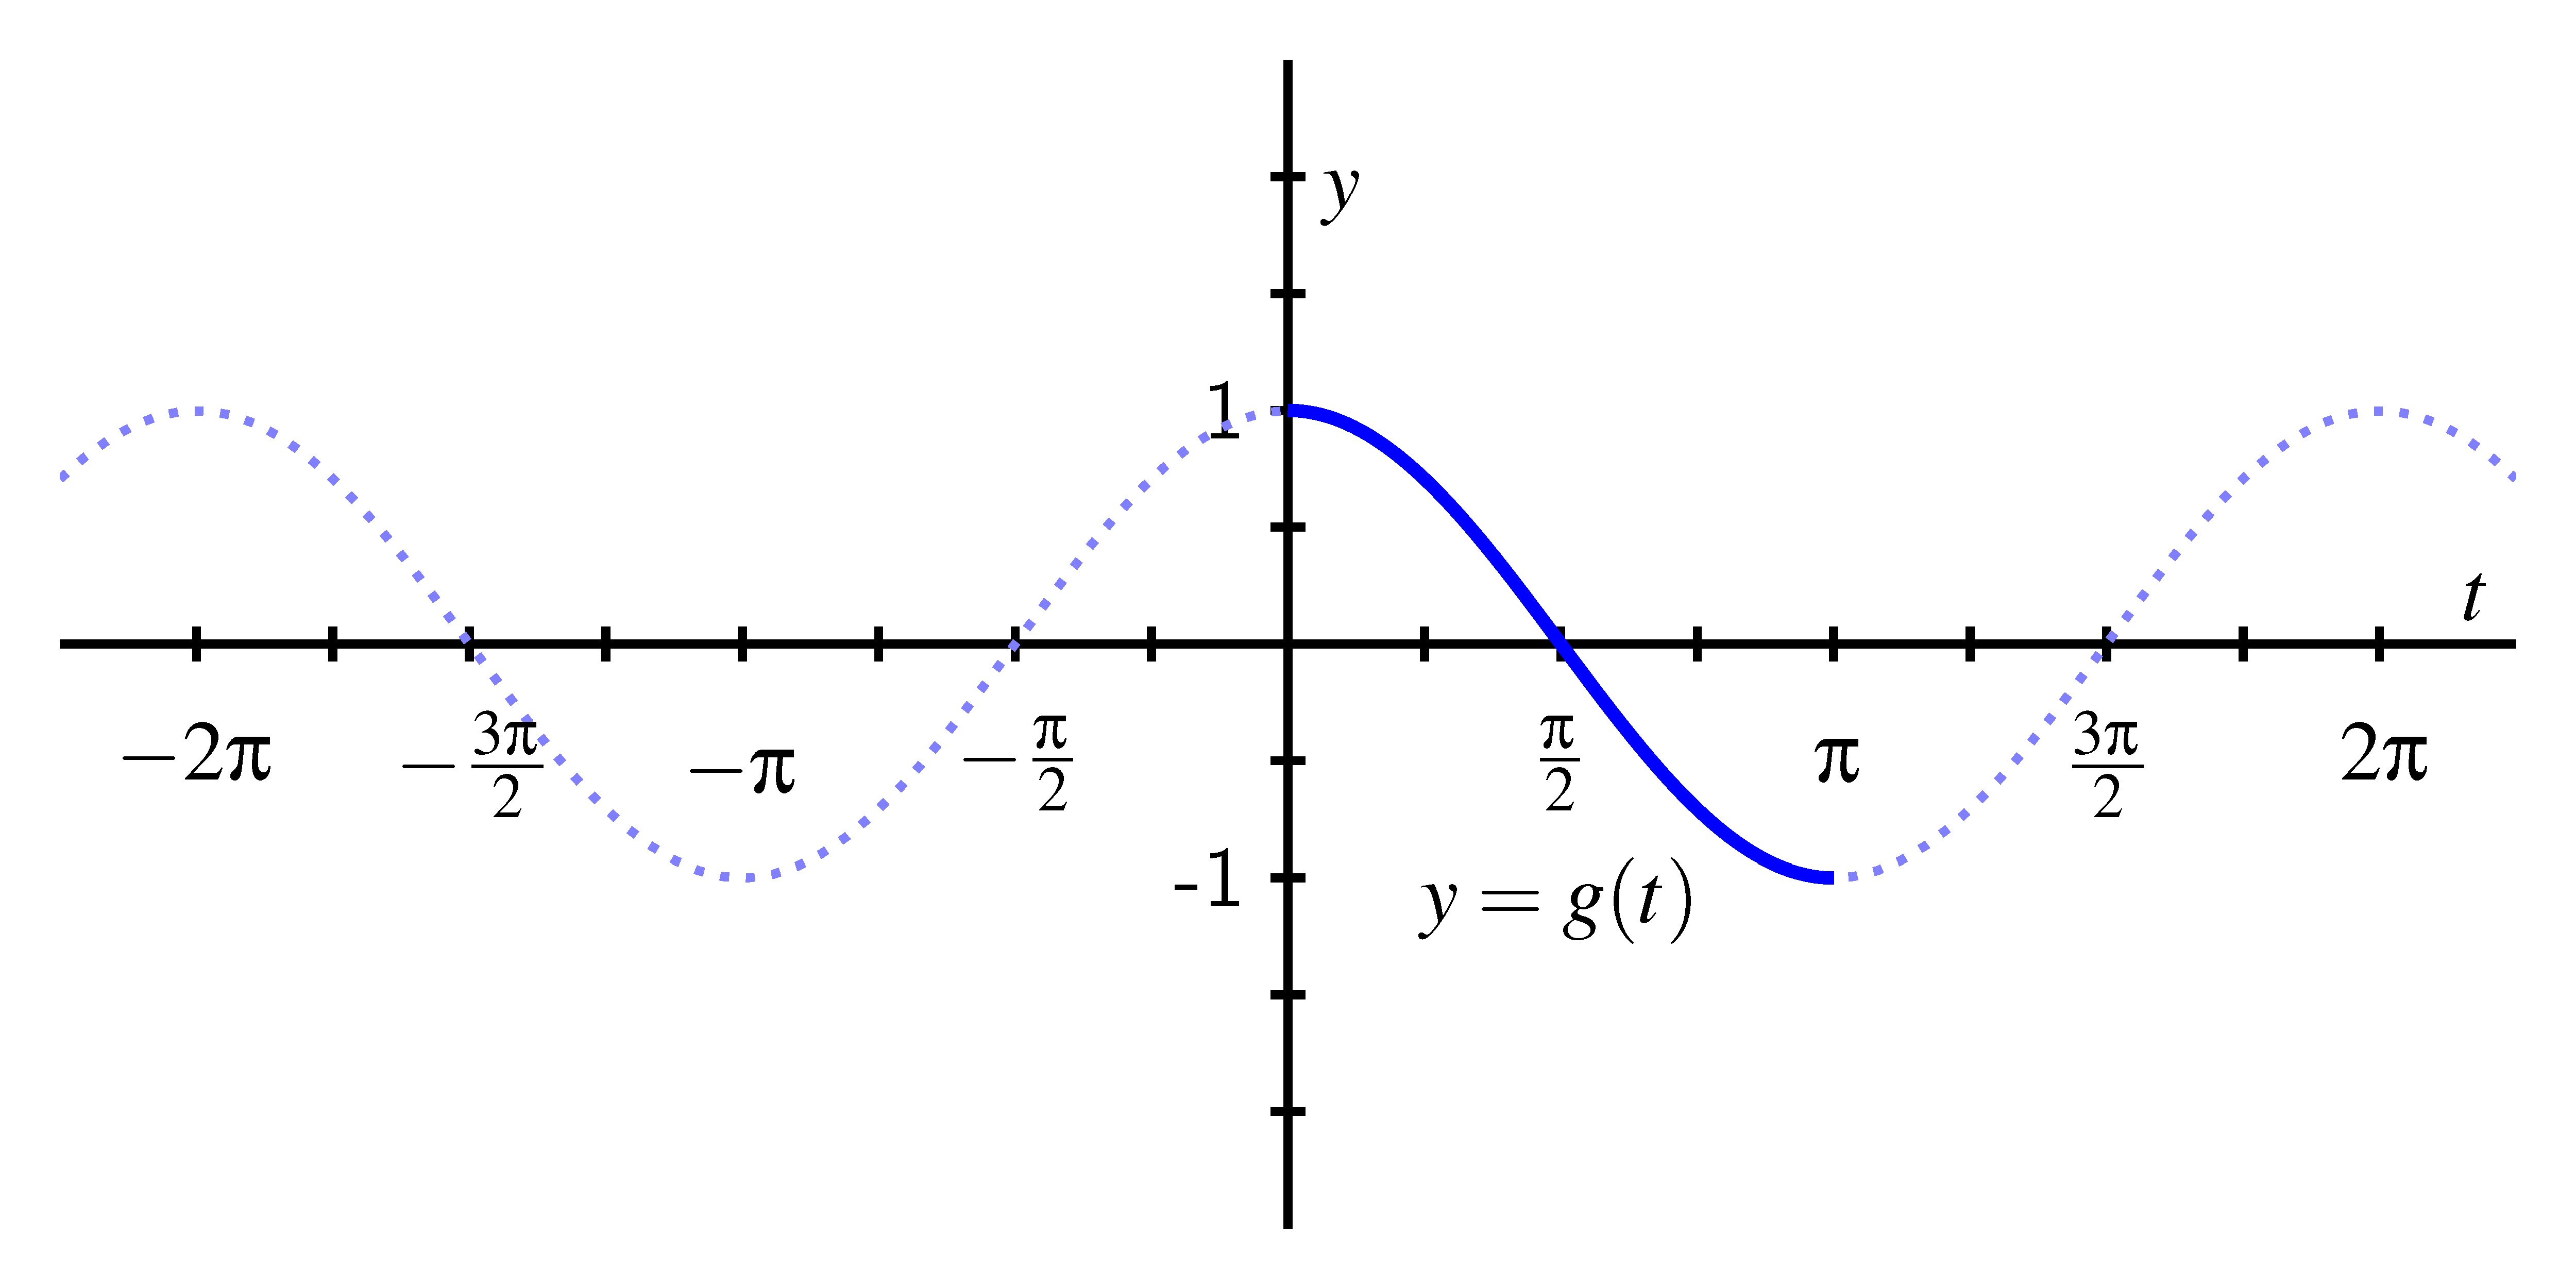
\includegraphics{inverse-trig-PA-cosine.png}
%\end{image}

\end{explanation}

%=-\frac{\pi}{4}

\item $\arcsin(2x) = \frac{\pi}{3}$\\
\begin{explanation}
First, we observe that $\frac{\pi}{3}$ is in the range of arcsine, so there should be a solution. We will now use the fact that sine is the inverse of arcsine to reduce this to a linear equation.
\begin{align*}
\arcsin(2x) &= \frac{\pi}{3}\\
\sin(\arcsin(2x)) &= \sin\left(\frac{\pi}{3}\right) \\
\end{align*}
Thus, we have
$$2x = \frac{\sqrt{3}}{2},$$
which is equivalent to $x = \frac{\sqrt{3}}{4}$.

\end{explanation}
\end{enumerate}
\end{example}

\section{The Arctangent Function}
Next, we develop an inverse function for a restricted version of the tangent function.  We choose the domain $\Big(\!-\frac{\pi}{2}, \frac{\pi}{2}\Big)$ on which $h(t) = \tan(t)$ is increasing and attains all of the values in the range of the tangent function.%
\begin{definition}
Let $y = h(t) = \tan(t)$ be defined on the domain $\Big(\!-\frac{\pi}{2}, \frac{\pi}{2}\Big)$, and observe $h$ has the range $\big(-\infty,\infty\big)$.  For any real number $y$, the \dfn{arctangent of $\mathbf{y}$}, denoted%
\begin{equation*}
\arctan(y)
\end{equation*}
is the angle $t$ satisfying $-\frac{\pi}{2} < t <  \frac{\pi}{2}$ such that $\tan(t) = y$.
%
Note that we use $t=\tan^{-1}(y)$ interchangeably with with $t = \arctan(y)$. 
\end{definition}

\begin{problem}
Let us once again channel our inner Sherlock Holmes to understand key properties of the arctangent function.%
\par
\begin{enumerate}
\item Using the definition given above, what are the domain and range of the arctangent function?
%
\begin{itemize}
\item The domain of arctangent is $(\answer{-\infty} , \answer{\infty})$.
%
\item The range of arctangent is $\Big(\answer{-\frac{\pi}{2}} , \answer{\frac{\pi}{2}} \Big)$.
\end{itemize}
%
\item Determine the following values exactly: 
\begin{itemize}
\item $\arctan(-\sqrt{3}) = \answer{\frac{\pi}{3}}$
%
\item $\arctan(-1) = \answer{-\frac{\pi}{4}}$
%
\item $\arctan(0) = \answer{0}$
%
\item $\arctan\!\Big(\frac{1}{\sqrt{3}}\Big) = \answer{\frac{\pi}{6}}$.
\end{itemize}
%
\item The restricted tangent function on the interval $\Big(\!-\frac{\pi}{2}, \frac{\pi}{2}\Big)$ is plotted below. On the same axes, sketch its corresponding inverse function (arctangent).  Label at least three points on each curve so that each point on the tangent graph corresponds to a point on the arctangent graph. In addition, sketch the line $y = t$ to demonstrate how the graphs are reflections of one another across this line.%
%
\item Complete the following sentence:  ``as $t$ increases without bound, $\arctan(t)$ $\ldots$'' \wordChoice{\choice{increases without bound}\choice{decreases without bound}\choice[correct]{increases toward $\frac{\pi}{2}$}\choice{decreases toward $-\frac{\pi}{2}$}}%
\end{enumerate}
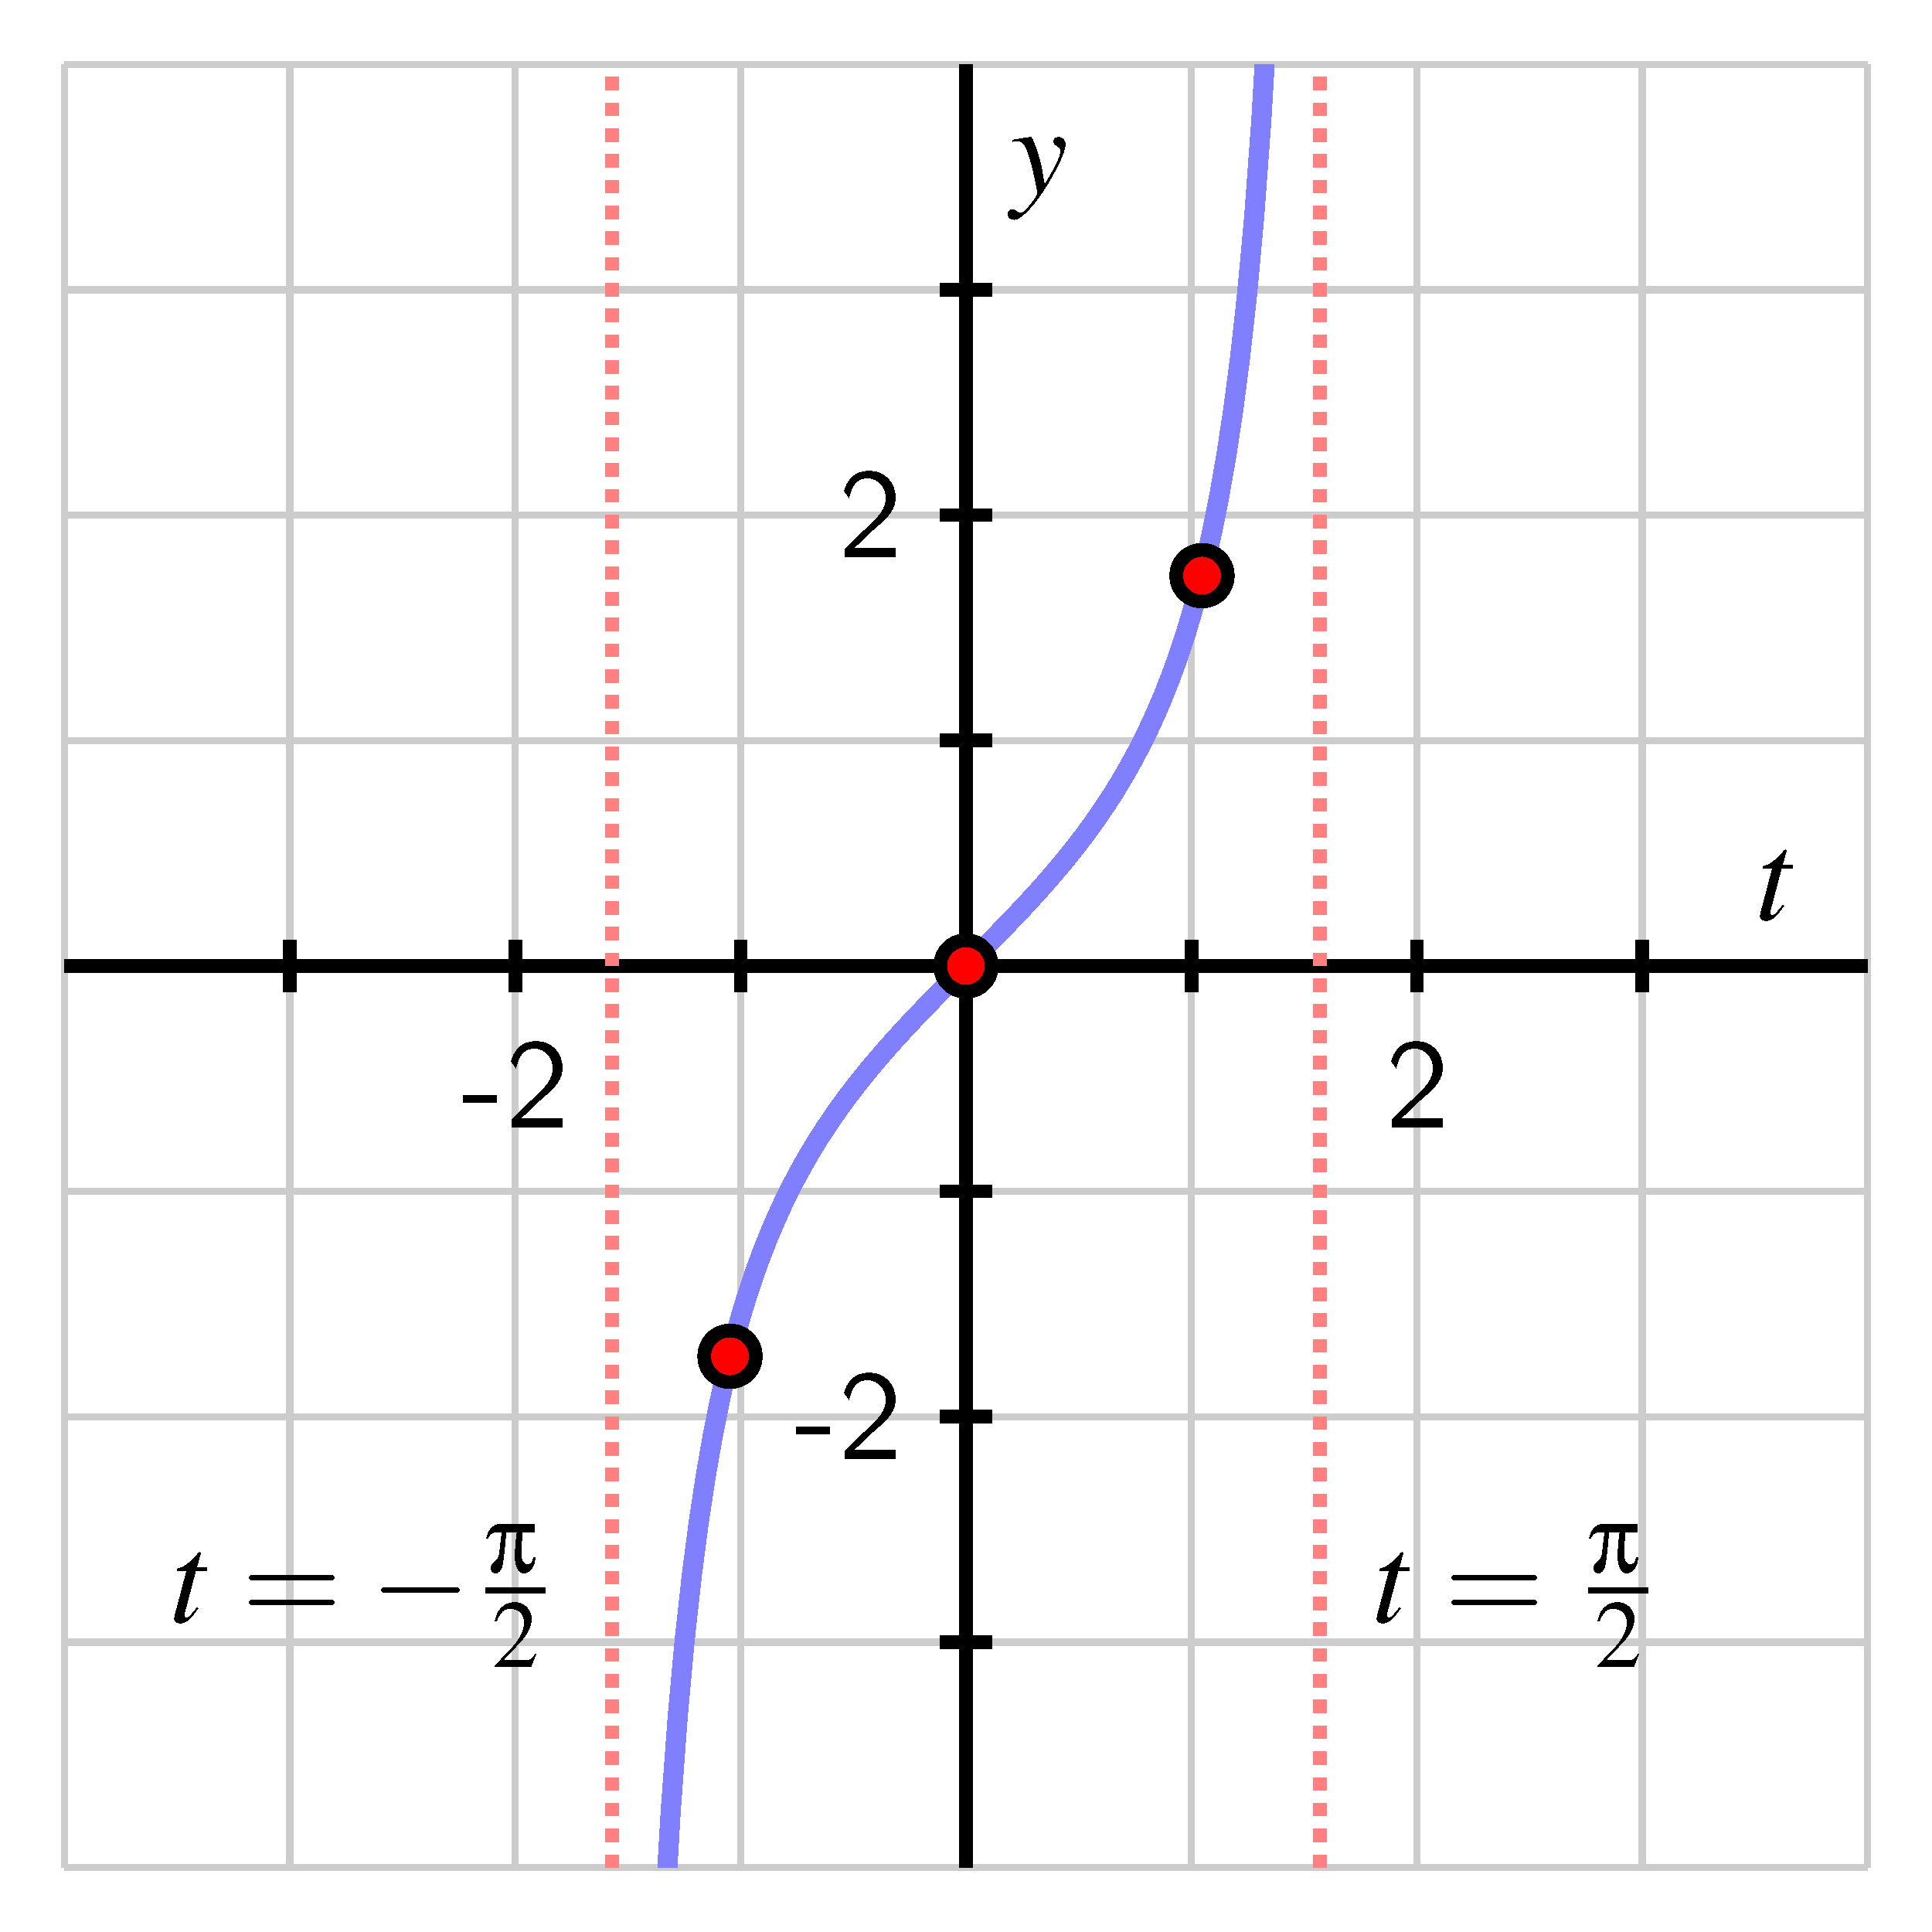
\includegraphics[width=1\linewidth]{inverse-tan-graph.png}
\end{problem}

\begin{callout}{\bf Properties of the arctangent function.}%
\begin{itemize}
\item
The restricted tangent function, $y = h(t) = \tan(t)$, is defined on the domain $\Big(\!\!-\frac{\pi}{2}, \frac{\pi}{2}\Big)$ with range $(-\infty,\infty)$.  This function has an inverse function that we call the arctangent function, denoted $t = h^{-1}(y) = \arctan(y)$.%
\item
The domain of $y = h^{-1}(t) = \arctan(t)$ is $(-\infty,\infty)$ with range $\Big(\!\!-\frac{\pi}{2}, \frac{\pi}{2}\Big)$.%
\item
The arctangent function is always increasing on its domain.%
\item
Below we have a plot of the restricted tangent function (in light blue) and its corresponding inverse, the arctangent function (in dark blue).%
\end{itemize}
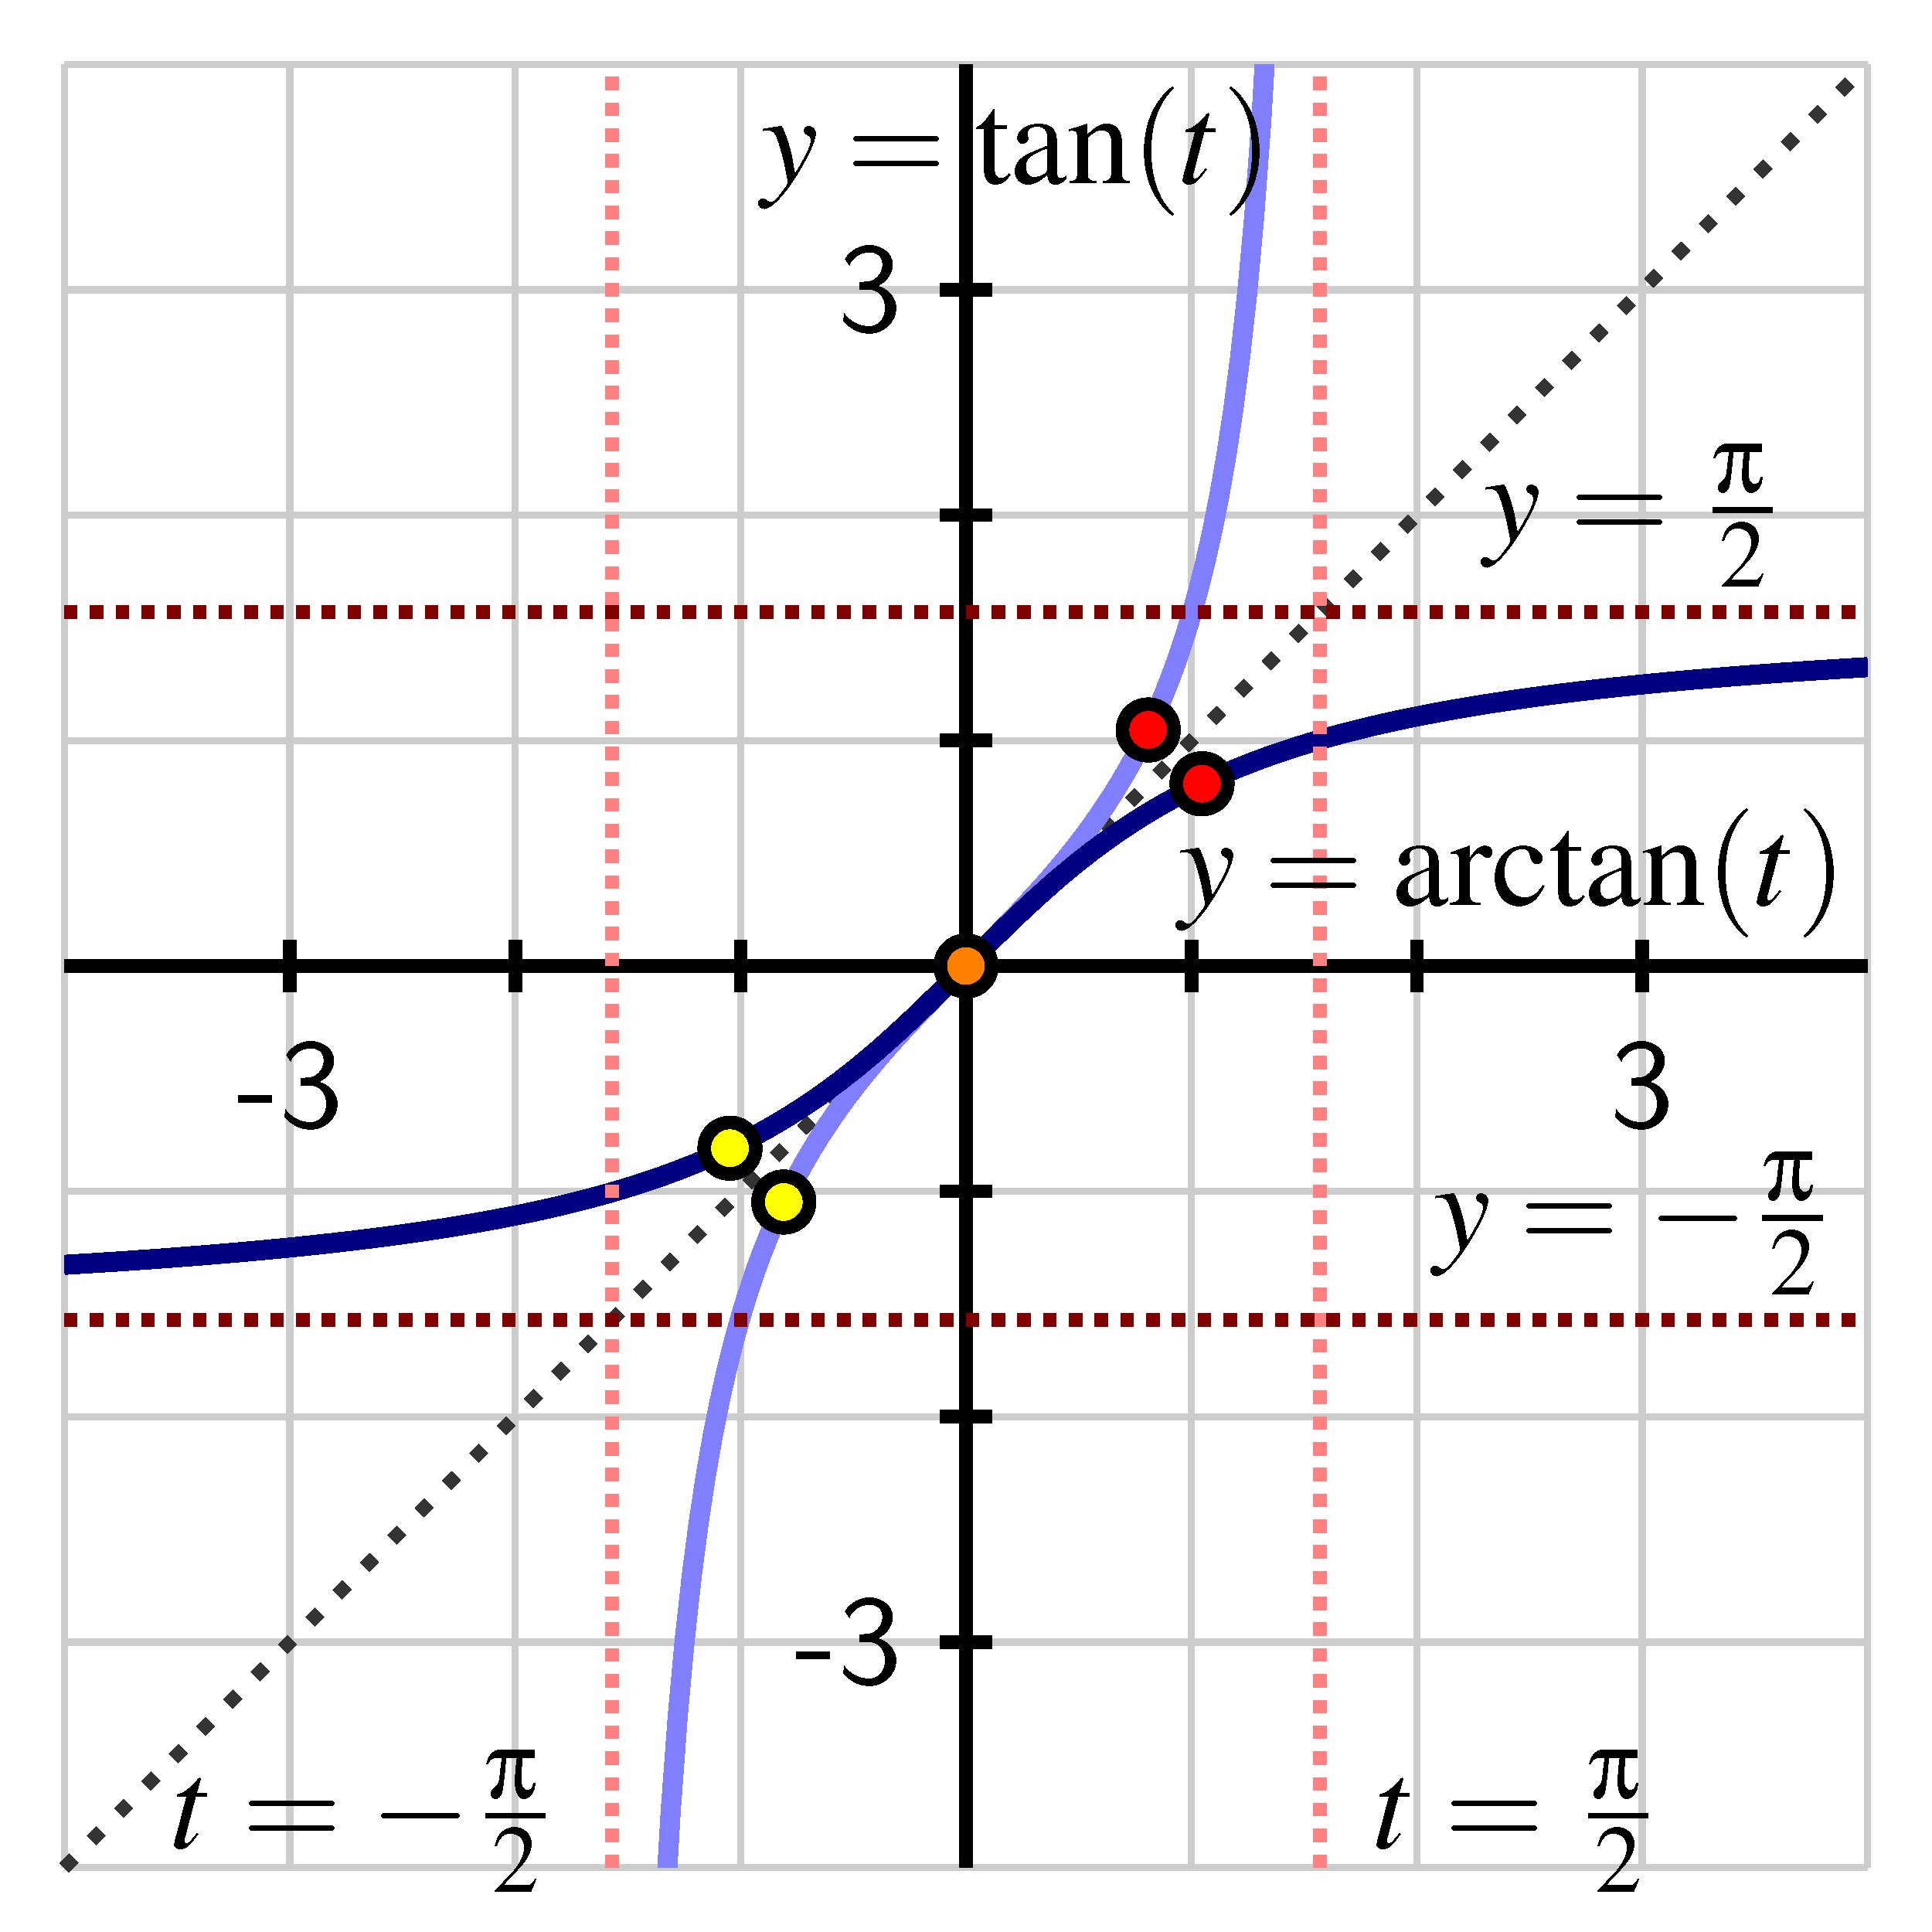
\includegraphics[width=1\linewidth]{inverse-trig-arctan-graph.png}
\end{callout}

\section{Exploring Arctangent}

\begin{example}
Let's solve the following equations analytically, then we can consider the graph of arctangent.	
\begin{enumerate}
%
\item $\tan(\arctan(-\sqrt{3}))$\\
\begin{explanation}
We start by finding $\arctan(-\sqrt{3})$. Remember that for $x$ in $(-\infty,\infty)$, $\arctan(x)$ is the value $y$ in $\Big(\!-\frac{\pi}{2},\frac{\pi}{2}\Big)$ such that $\tan(y) = x$. 

Hence, $y$ is $-\frac{\pi}{3}$, and we now see that 
\begin{equation*}
\tan(\arctan(-\sqrt{3})) = \tan\Big(\!-\frac{\pi}{3}\Big) = -\sqrt{3}.
\end{equation*}

Now, I know you're thinking, ``Hey, why do you keep making us do an extra step?" It's because it is imperative that you \textbf{\textit{consider the range}} of the arc trig functions. These are considerations you will also need to make when we start combining different trig functions with the inverses of others (say sine of arctangent of a value).

Let's recall how we defined arctangent. Since tangent is a periodic function, it fails the horizontal line test. However, if we {\it restrict} tangent to a single period (note tangent only increasing), $\Big(\!-\frac{\pi}{2},\frac{\pi}{2}\Big)$, then we may define a function $h$ on this domain such that $h(x) = \tan(x)$ for $x$ in $\Big(\!-\frac{\pi}{2},\frac{\pi}{2}\Big)$. Arctangent then is defined as the inverse of this function $h$. Therefore, $h$ is the inverse of arctangent. 
Thus, in practice, tangent is the inverse of arctangent. 

A word of caution: As was the case with the previous two trig functions and their respective inverses, arctangent is only the inverse of restricted tangent. We will illustrate this with the next example.
\end{explanation}

%=-\sqrt{3}

\item $\arctan\!\Big(\!\tan\!\Big(\frac{5\pi}{3}\Big)\Big)$

\begin{explanation}
It may be tempting to take a look at this expression and conclude that the solution is $\frac{5\pi}{3}$ since arctangent is the inverse of tangent. 

{\bf But, wait! }

Remember, we had to restrict the domain of tangent in order to define an inverse function, which we called arctangent. Arctangent is the inverse of the {\it restricted} tangent function, whose domain is $\Big(\!-\frac{\pi}{2},\frac{\pi}{2}\Big)$. $\frac{5\pi}{3}$ is larger than $\frac{\pi}{2}$, so it is not within the domain of this restricted tangent function. 

Thus, we begin by simplifying $\tan\!\Big(\frac{5\pi}{3}\Big) = -\sqrt{3}$. 

Now, let's consider $\arctan(-\sqrt{3})$, recalling again the {\it range} of arctangent. We are looking for the value of $y$ in $\Big(\!-\frac{\pi}{2},\frac{\pi}{2}\Big)$ such that $\tan(y) =-\sqrt{3}$.

Hence, $y$ is $-\frac{\pi}{3}$, and we now see that 
\begin{equation*}
\arctan\!\Big(\!\tan\!\Big(\frac{5\pi}{3}\Big)\Big) = \arctan(-\sqrt{3}) = -\frac{\pi}{3}.
\end{equation*}

%Now, let's look again at the graph of cosine. Here we highlight $g: [0,\pi] \rightarrow [0,\pi]$ defined by $y=g(x)=\cos(x)$, the restricted cosine function. We may use the symmetry of the graph of cosine to help find the appropriate values for arccosine.
%\begin{image}
%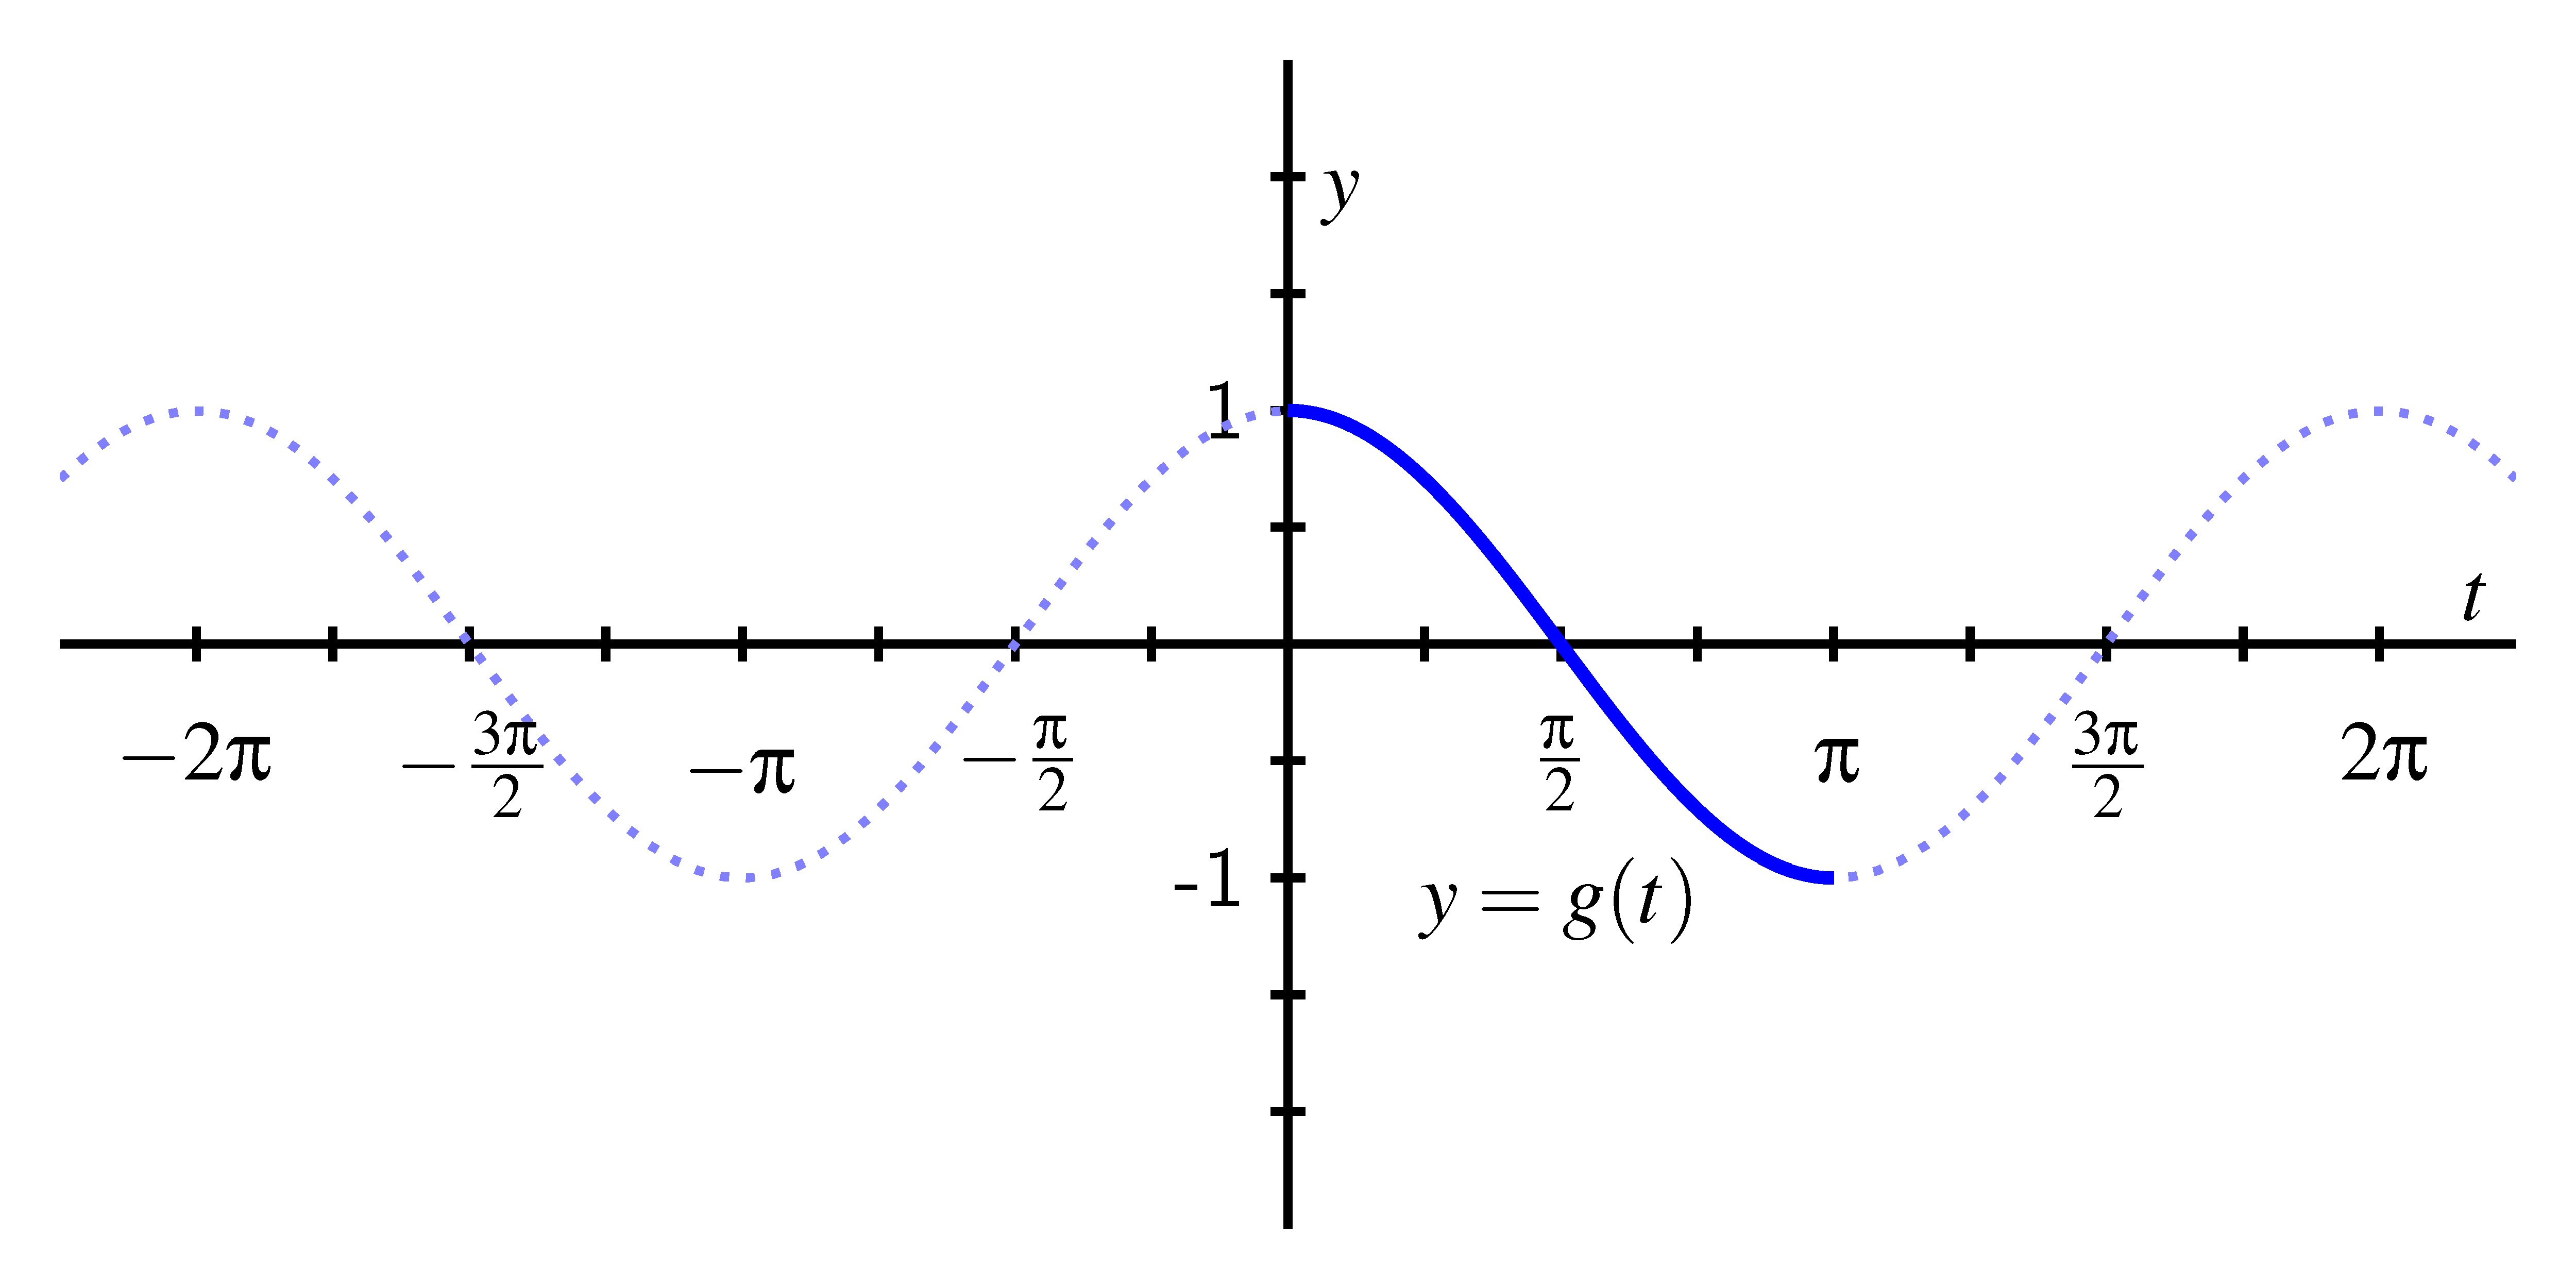
\includegraphics{inverse-trig-PA-cosine.png}
%\end{image}

\end{explanation}

% = -\frac{\pi}{3}$

\item $4\arctan^2(x) - 3\pi \arctan(x) - \pi^2 = 0$\\
\begin{explanation}
	We will treat this like a quadratic equation to begin, as we did in the section Some Applications of Trig Functions. 

Let $y = \arctan(x)$, then we have a standard quadratic equation: $4y^2- 3\pi y - \pi^2=0$. Factoring, we see that this is equivalent to 
$$(4y +\pi)(y-\pi)=0.$$
%
This has two solutions: $y = -\frac{\pi}{4}$ and $y=\pi$. In other words, we now simply solve (a) $\arctan(x) = -\frac{\pi}{4}$ and (b) $\arctan(x) = \pi$. $\pi$ is not in the range of arctangent, so (b) does not have a solution. Hence, this cannot be a solution to our equation, and we must look at (a). $-\frac{\pi}{4}$ is in the range of arctangent, so the solution to (a) will be a solution to our original equation.

Since tangent is the inverse to arctangent, the equation (a) is equivalent to $$\tan(\arctan(x))=\tan\!\Big(\!-\frac{\pi}{4}\Big),$$
which is further equivalent to $x=-1$
\end{explanation}
\end{enumerate}
\end{example}

%%%%%%%%%%%%%%%%%%%ARCSECANT
\section{The Arcsecant Function}
%
We will also consider the inverse function for a restricted version of the secant function. 
As with the cosine and sine functions, we need to choose an interval on which the secant function is always increasing or always decreasing in order to have the function pass the horizontal line test. In the case of secant, this means choosing two distinct intervals. A word of caution in working with the restricted secant function and its associated inverse, there is not a ``standard" choice for the domain of restricted secant. {\it However}, we will establish a convention in this course. 

We restrict the domain of the function $k(t) = \sec(t)$ to $[0,\pi/2) \cup (\pi/2,\pi ]$, where secant is increasing on each interval and attains all the values within the range of the secant function. By reflecting across the line $y=t$ and switching the $t$ and $y$ coordinates we are able to define the function $k^{-1}(t)=\arcsec(t)$ as follows.

\begin{definition}
Let $y = k(t) = \sec(t)$ be defined on the domain $[0,\pi/2) \cup (\pi/2,\pi ]$, and observe that $k$ has the range $(-\infty,-1] \cup [1,\infty)$. 
For any real number $y$, the {\bf arcsecant of y}, denoted
$$\arcsec(y)$$
is the angle $t$ satisfying $0 \leq t < \frac{\pi}{2}$ or $\frac{\pi}{2} < t \leq \pi$. Note that we use $t = \sec^{-1}(y)$ interchangeably with $t = \arcsec(y)$.
\end{definition}

\begin{problem}
Take the lead Watson, and we will deduce the key properties of the arcsecant function as we did above for arcsine and arctangent.
\begin{enumerate}
\item
Using the definition of arcsecant given above, what are the domain and range of the arcsecant function? \\
\begin{itemize}
\item The domain of arcsecant is $(\answer{-\infty} , \answer{-1}] \cup [\answer{1} , \answer{\infty})$.
%
\item The range of arcsecant is $\Big[\answer{0} , \answer{\frac{\pi}{2}}\Big) \cup \Big(\answer{\frac{\pi}{2}} , \answer{\pi}\Big]$.
\end{itemize}
%
\item Determine the following values exactly: 
\begin{itemize}
%
\item $\arcsec(1) = \answer{0}$
%
\item $\arcsec(-1) = \answer{\pi}$
%
\item $\arcsec(2) = \answer{\frac{\pi}{3}}$ 
%\item $\arcsin\Big(\frac{\sqrt{3}}{2}\Big) = \answer{\frac{\pi}{3}}$
\end{itemize}
%
\item
On the axes provided below, sketch a careful plot of the restricted secant function on the intervals $\Big[0, \frac{\pi}{2}\Big)$ and $\Big(\frac{\pi}{2}, \pi\Big]$ along with its corresponding inverse, the arcsecant function.  Label at least three points on each curve so that each point on the secant graph corresponds to a point on the arcsecant graph.  %In addition, sketch the line $y = t$ to demonstrate how the graphs are reflections of one another across this line.

%Can we get axes with $\pm 1$ and $\pi$ and $\frac{\pi}{2}$ labeled?
%
%
\item True or false: $\arcsec(\sec(2\pi)) = 2\pi$? \wordChoice{\choice{true}\choice[correct]{false}} \\
Write a complete sentence to explain your reasoning.%
\end{enumerate}

\begin{image}
\includegraphics[width=1\linewidth]{SecArcsecAxis.png}
\end{image}
\end{problem}

\begin{callout}{\bf Properties of the arcsecant function.}%
\begin{itemize}
\item
The restricted secant function, $y = k(t) = \sec(t)$, is defined on the domain $\Big[0,\frac{\pi}{2}\Big) \cup \Big(\frac{\pi}{2},\pi \Big]$ with range $(-\infty, -1] \cup [1,\infty)$.  This function has an inverse function that we call the arcsecant function, denoted $t = k^{-1}(y) = \arcsec(y)$.
%
\item
The domain of $y = k^{-1}(t) = \arcsec(t)$ is $(-\infty, -1] \cup [1,\infty)$ with range $\Big[0,\frac{\pi}{2}\Big) \cup \Big(\frac{\pi}{2},\pi \Big]$.
%
\item
The arcsecant function is always increasing on each interval in its domain.
%
\item Recall that $\sec(\theta) = \frac{1}{\cos(\theta)}$. Arcsecant and arccosine maintain a relationship as well, though they are {\it not} reciprocals: \\
For $t$ in the domain of arcsecant, $\arcsec(t) = \arccos\!\Big(\frac{1}{t}\Big)$.
%
%
% %\includegraphics[width=1\linewidth]{arcsecantGraph.png}
% 
%  \includegraphics[width=1\linewidth]{arcsecantGraph2.png}
%
%CODE FROM STITZ ZEAGER...not sure how to make this work: 
% \[ \begin{array}{ccc}
%
%\begin{mfpic}[25][20]{-0.5}{4}{-4}{4}
%\point[3pt]{(0,1), (3.1416, -1)}
%\axes
%\tlabel[cc](4,-0.25){\scriptsize $x$}
%\tlabel[cc](0.25,4){\scriptsize $y$}
%\tcaption{\scriptsize  $f(x) = \sec(x)$ on  $\left[0, \frac{\pi}{2}\right) \cup \left( \frac{\pi}{2}, \pi\right]$}
%\xmarks{1.5708, 3.1416}
%\ymarks{-1,1}
%\tlpointsep{4pt}
%\axislabels {x}{{\scriptsize $\frac{\pi}{2}$} 1.5708,  {\scriptsize $\pi$} 3.1416}
%\axislabels {y}{{\scriptsize $-1$} -1, { \scriptsize $1$} 1}
%\dashed \polyline{(1.5708, -4), (1.5708, 4)}
%\arrow \function{0, 1.3181, 0.1}{1/cos(x)}
%\arrow  \reverse  \function{1.8235, 3.1416, 0.1}{1/cos(x)}
%\end{mfpic}
%
%&
%
%\stackrel{\stackrel{\mbox{\scriptsize reflect across $y=x$}}{\xrightarrow{\hspace{1in}}}}{\mbox{ \scriptsize switch $x$ and $y$ coordinates}} 
%
%&
%
%\begin{mfpic}[20][25]{-4}{4}{-0.5}{4}
%\point[3pt]{(1,0), (-1,3.1416)}
%\axes
%\tlabel[cc](4,-0.25){\scriptsize $x$}
%\tlabel[cc](0.25,4){\scriptsize $y$}
%\tcaption{\scriptsize  $f^{-1}(x) = \mbox{arcsec}(x)$}
%\ymarks{1.5708, 3.1416}
%\xmarks{-1,1}
%\tlpointsep{4pt}
%\axislabels {y}{{\scriptsize $\frac{\pi}{2}$} 1.5708,  {\scriptsize $\pi$} 3.1416}
%\axislabels {x}{{\scriptsize $-1 \hspace{7pt}$} -1, { \scriptsize $1$} 1}
%\dashed \polyline{(-4, 1.5708), (4, 1.5708)}
%\arrow \parafcn{0, 1.3181, 0.1}{(1/cos(t),t)}
%\arrow  \reverse  \parafcn{1.8235, 3.1416, 0.1}{(1/cos(t),t)}
%\end{mfpic}
%
%\end{array}\]
%Below we have a plot of the restricted tangent function (in light blue) and its corresponding inverse, the arctangent function (in dark blue).%
\end{itemize}
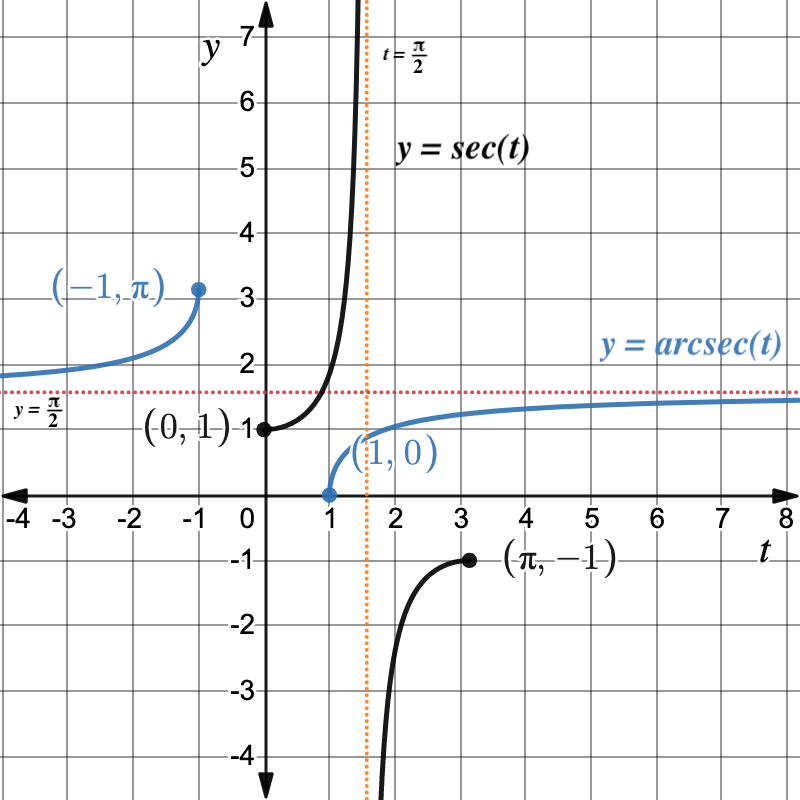
\includegraphics[width=1\linewidth]{secArcsecGraphst.png}
\end{callout}

\section{Exploring Arcsecant} 

\begin{example}
Sometimes we must rely on other properties of these functions and their relations to more familiar functions to find solutions. In the following examples, we wish to find $x$ in the range of arcsecant such that
\begin{enumerate}
\item $x = \arcsec(-\sqrt{2})$ \\
\begin{explanation}
We may use the relationship between arcsecant and arccosine to rewrite this equation in terms of arccosine. In other words, since $\arcsec(y) = \arccos\!\Big(\frac{1}{y}\Big)$, for $y$ in the domain of arcsecant,
$$\arcsec(-\sqrt{2}) = \arccos\!\Big(\!\!-\frac{\sqrt{2}}{2}\Big) = \frac{3\pi}{4}.$$
\end{explanation}

\item $x=\arcsec \!\Big(\!\! - \frac{2\sqrt{3}}{3}\Big)$\\
\begin{explanation}
Again, we use the relationship $\arcsec(y) = \arccos\!\Big(\frac{1}{y}\Big)$, for $y$ in the domain of arcsecant:
%
$$\arcsec \!\Big(\!\! - \frac{2\sqrt{3}}{3}\Big) = \arccos\!\Big(\!\! - \frac{\sqrt{3}}{2}\Big),$$
%
since the reciprocal of $\frac{2\sqrt{3}}{3} = \frac{3}{2\sqrt{3}} = \frac{\sqrt{3}}{2}$. Thus, we have 
%
$$\arcsec \!\Big(\!\! - \frac{2\sqrt{3}}{3}\Big)=\frac{5\pi}{6}.$$
\end{explanation}

Let's consider a couple more traditional problems combining secant and arcsecant. Remember that we must be cautious of their respective domains and ranges as with combinations of sine and arcsine and tangent and cotangent explored above.
\item $\sec(\arcsec(-\sqrt{2}))$\\
\begin{explanation}
Recall from part (a), that we already solved the equation $x = \arcsec(-\sqrt{2})$, and found that $x = \frac{3\pi}{4}$. Hence, we can now plug that in to solve our current equation:
%
$$\sec(\arcsec(-\sqrt{2})) = \sec\!\Big(\frac{3\pi}{4}\Big) = -\sqrt{2}.$$
%
As we have observed previously with other trig inverses, we have $\sec(\arcsec(x)) = x$ for $x$ in the domain of arcsecant. However, we must be careful in our application of this, as exemplified by the next example.
\end{explanation}

\item $\arcsec\!\Big(\!\sec\!\Big(\frac{5\pi}{4}\Big)\Big)$\\
\begin{explanation}
Remember that we had to restrict the domain of secant in order to define the inverse function, arcsecant. Arcsecant is thus the inverse of the {\it restricted} secant function, which has domain $[0, \pi/2)\cup (\pi/2,\pi]$. Observing that $\frac{5\pi}{4} >\pi$, and is therefore not in the domain of the restricted secant function, we cannot simply treat arcsecant as the inverse.

Instead, we begin by finding $\sec\!\Big(\frac{5\pi}{4}\Big)$, which is equal to $-\sqrt{2}$.

We now have  $\arcsec\!\Big(\!\sec\!\Big(\frac{5\pi}{4}\Big)\Big) = \arcsec(-\sqrt{2})$, which we found to be equal to $\frac{3\pi}{4}$ in part (a). Thus, we may conclude that 
%
$$\arcsec\!\Big(\!\sec\!\Big(\frac{5\pi}{4}\Big)\Big) =\frac{3\pi}{4}.$$
\end{explanation}
\end{enumerate}
\end{example}

\begin{summary}
  %Often ends a section
  \begin{itemize}
\item We choose to define the restricted cosine, sine, tangent, and secant functions on the respective domains $[0,\pi]$, $[-\pi/2, \pi/2]$, $(-\pi/2, \pi/2)$, and $[0,\pi/2) \cup (\pi/2, \pi]$.
On each such interval, the restricted function is strictly decreasing (cosine) or strictly increasing (sine,  tangent, and secant), and thus has an inverse function.  The restricted sine and cosine functions each have range $[-1,1]$, while the restricted tangent's range is the set of all real numbers, and the restricted secant's range is $(-\infty,1] \cup [1,\infty)$. 
We thus define the inverse function of each as follows:%
%
\begin{enumerate}[label=\roman*.]
\item
For any $y$ such that $-1 \le y \le 1$, the arccosine of $y$ (denoted $\arccos(y)$) is the angle $t$ in the interval $[0,\pi]$ such that $\cos(t) = y$.  That is, $t$ is the angle whose cosine is $y$.
%
\item%
For any $y$ such that $-1 \le y \le 1$, the arcsine of $y$ (denoted $\arcsin(y)$) is the angle $t$ in the interval $[-\pi/2, \pi/2]$ such that $\sin(t) = y$.  That is, $t$ is the angle whose sine is $y$.
%
\item
For any real number $y$, the arctangent of $y$ (denoted $\arctan(y)$) is the angle $t$ in the interval $(-\pi/2, \pi/2)$ such that $\tan(t) = y$.  That is, $t$ is the angle whose tangent is $y$.
%
\item
For any real number $y$, the arcsecant of $y$ (denoted $\arcsec(y)$) is the angle $t$ in the interval $[0,\pi/2) \cup (\pi/2,\pi]$ such that $\sec(t) = y$.  That is, $t$ is the angle whose secant is $y$.%
\end{enumerate}
%
\item
%To discuss the properties of the three inverse trigonometric functions, we plot them on the same axes as their corresponding restricted trigonometric functions.  When we do so, we use $t$ as the input variable for both functions simultaneously so that we can plot them on the same coordinate axes.%
%\par
The domain of $y = g^{-1}(t) = \arccos(t)$ is $[-1,1]$ with corresponding range $[0,\pi]$, and the arccosine function is always decreasing.  These facts correspond to the domain and range of the restricted cosine function and the fact that the restricted cosine function is decreasing on $[0,\pi]$.
\begin{image}
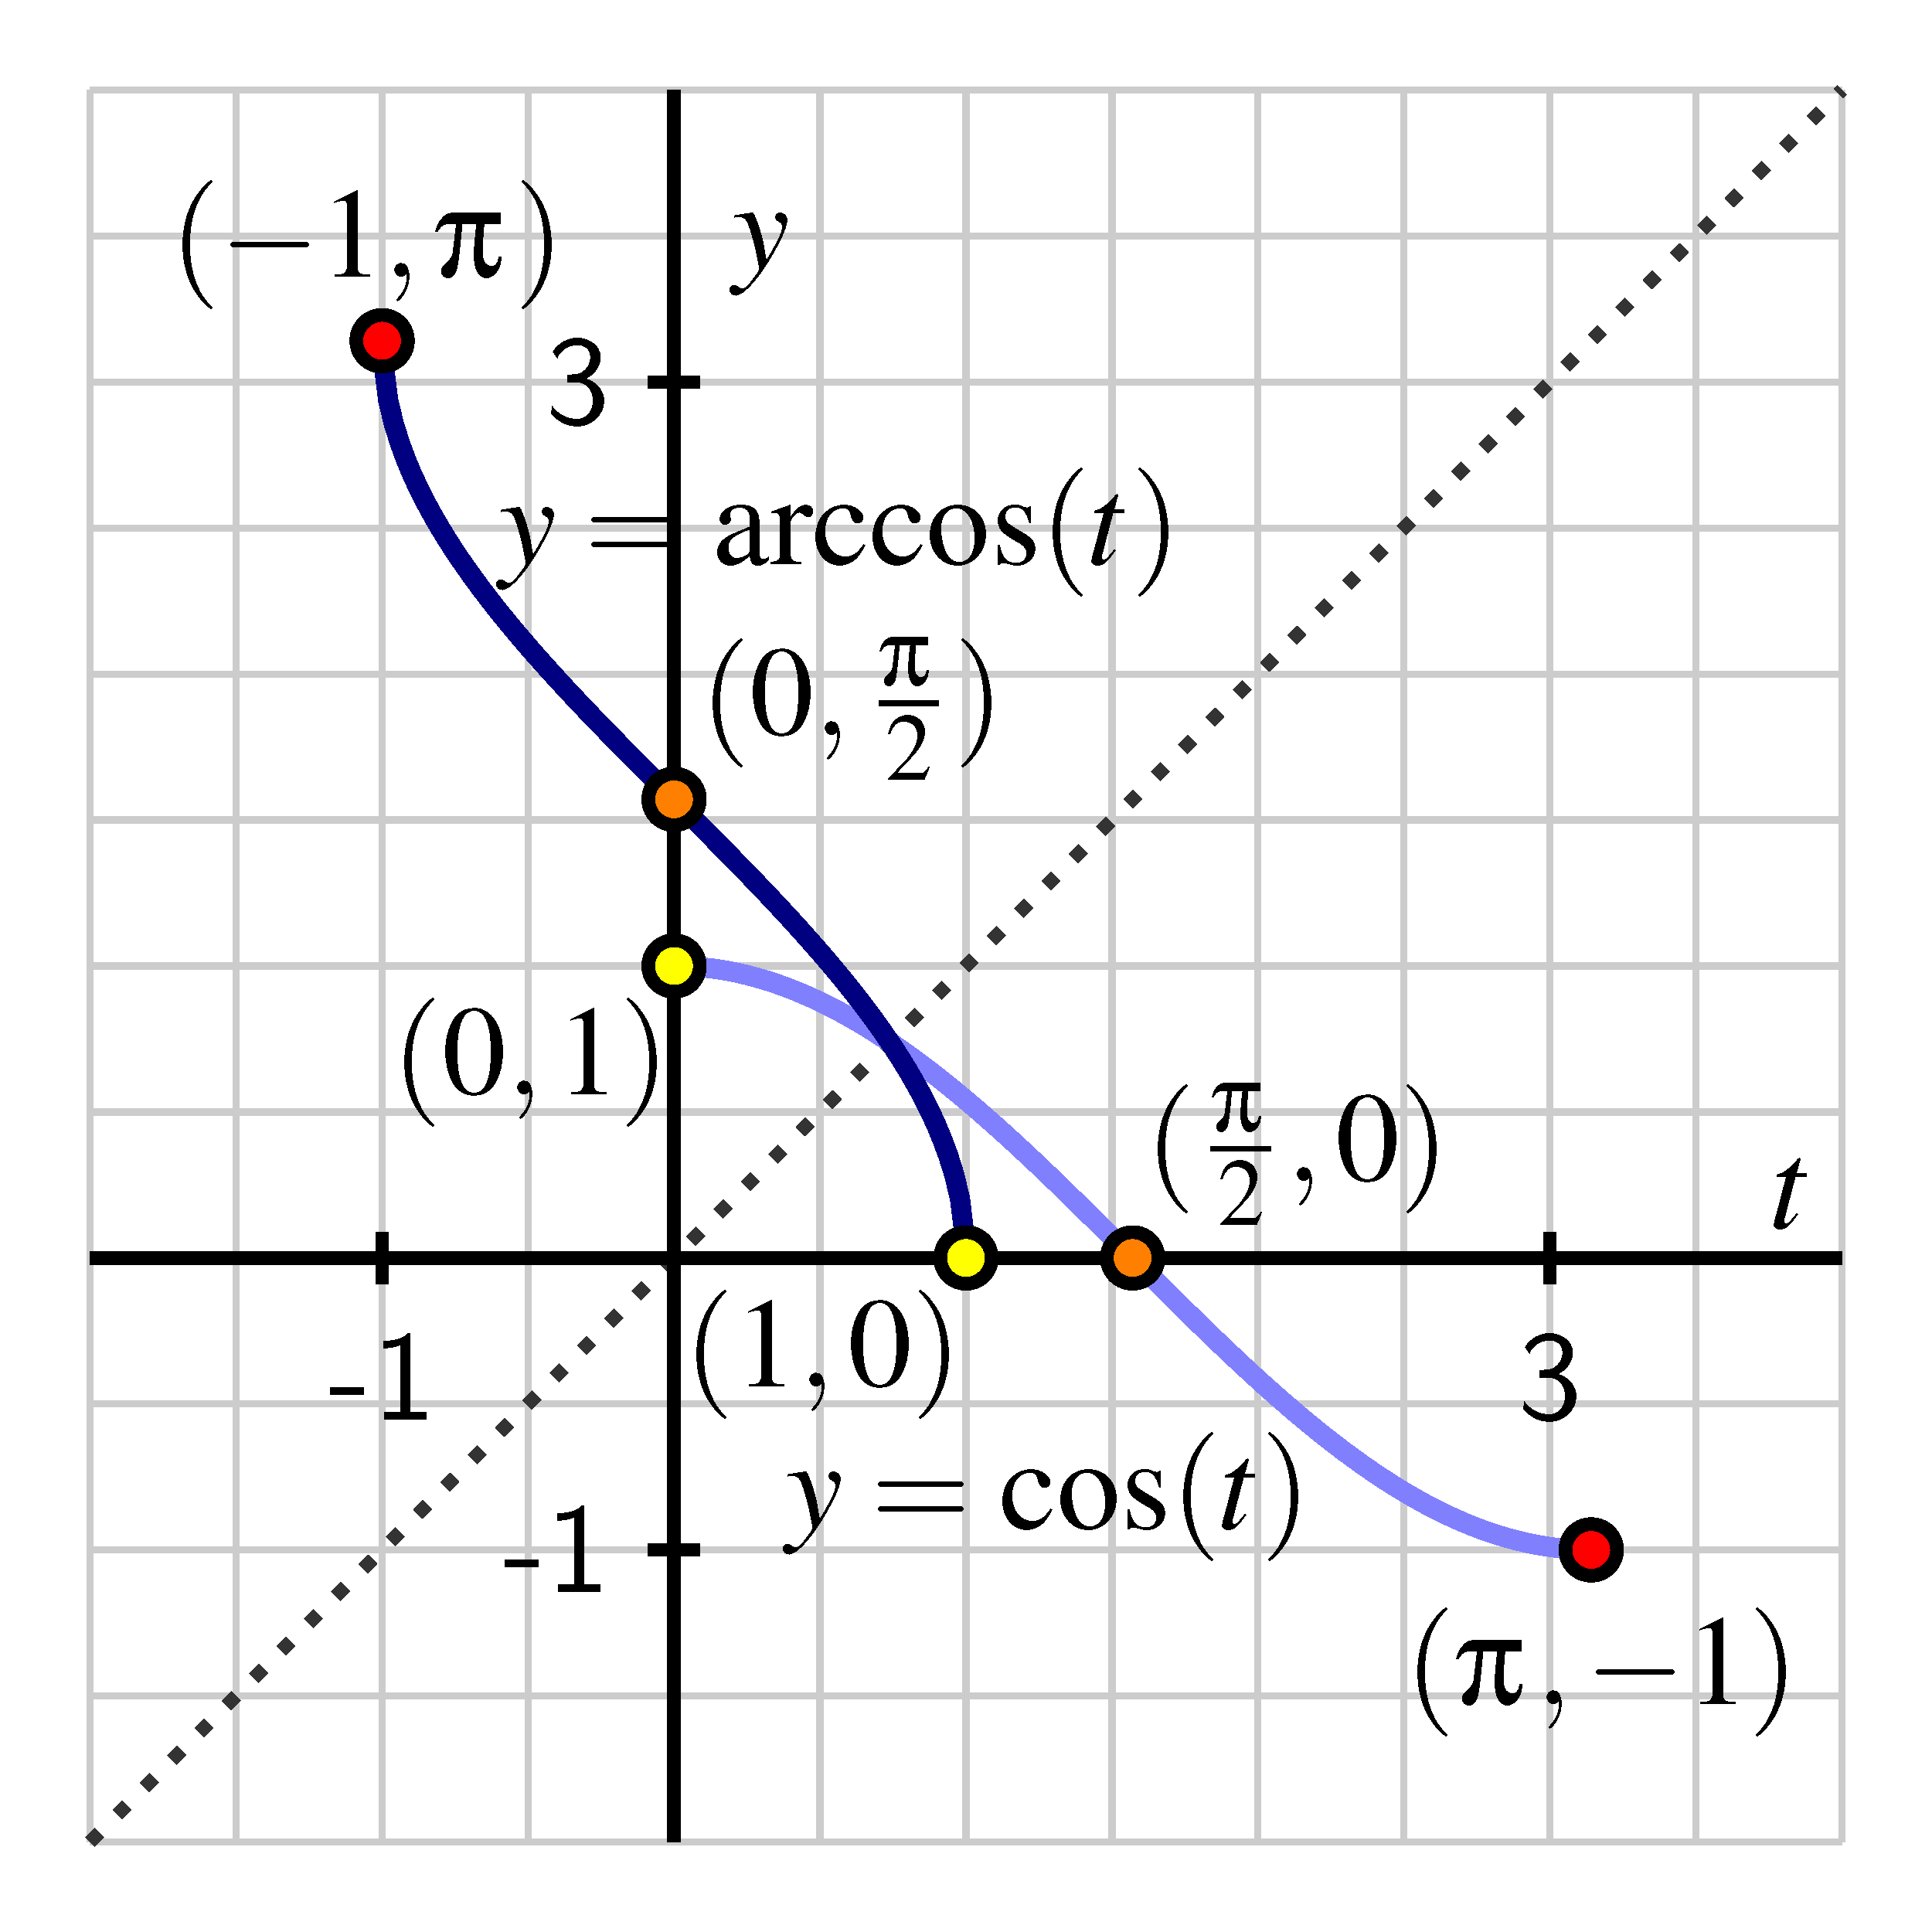
\includegraphics[width = .49\linewidth]{inverse-trig-arccos-graph.png}
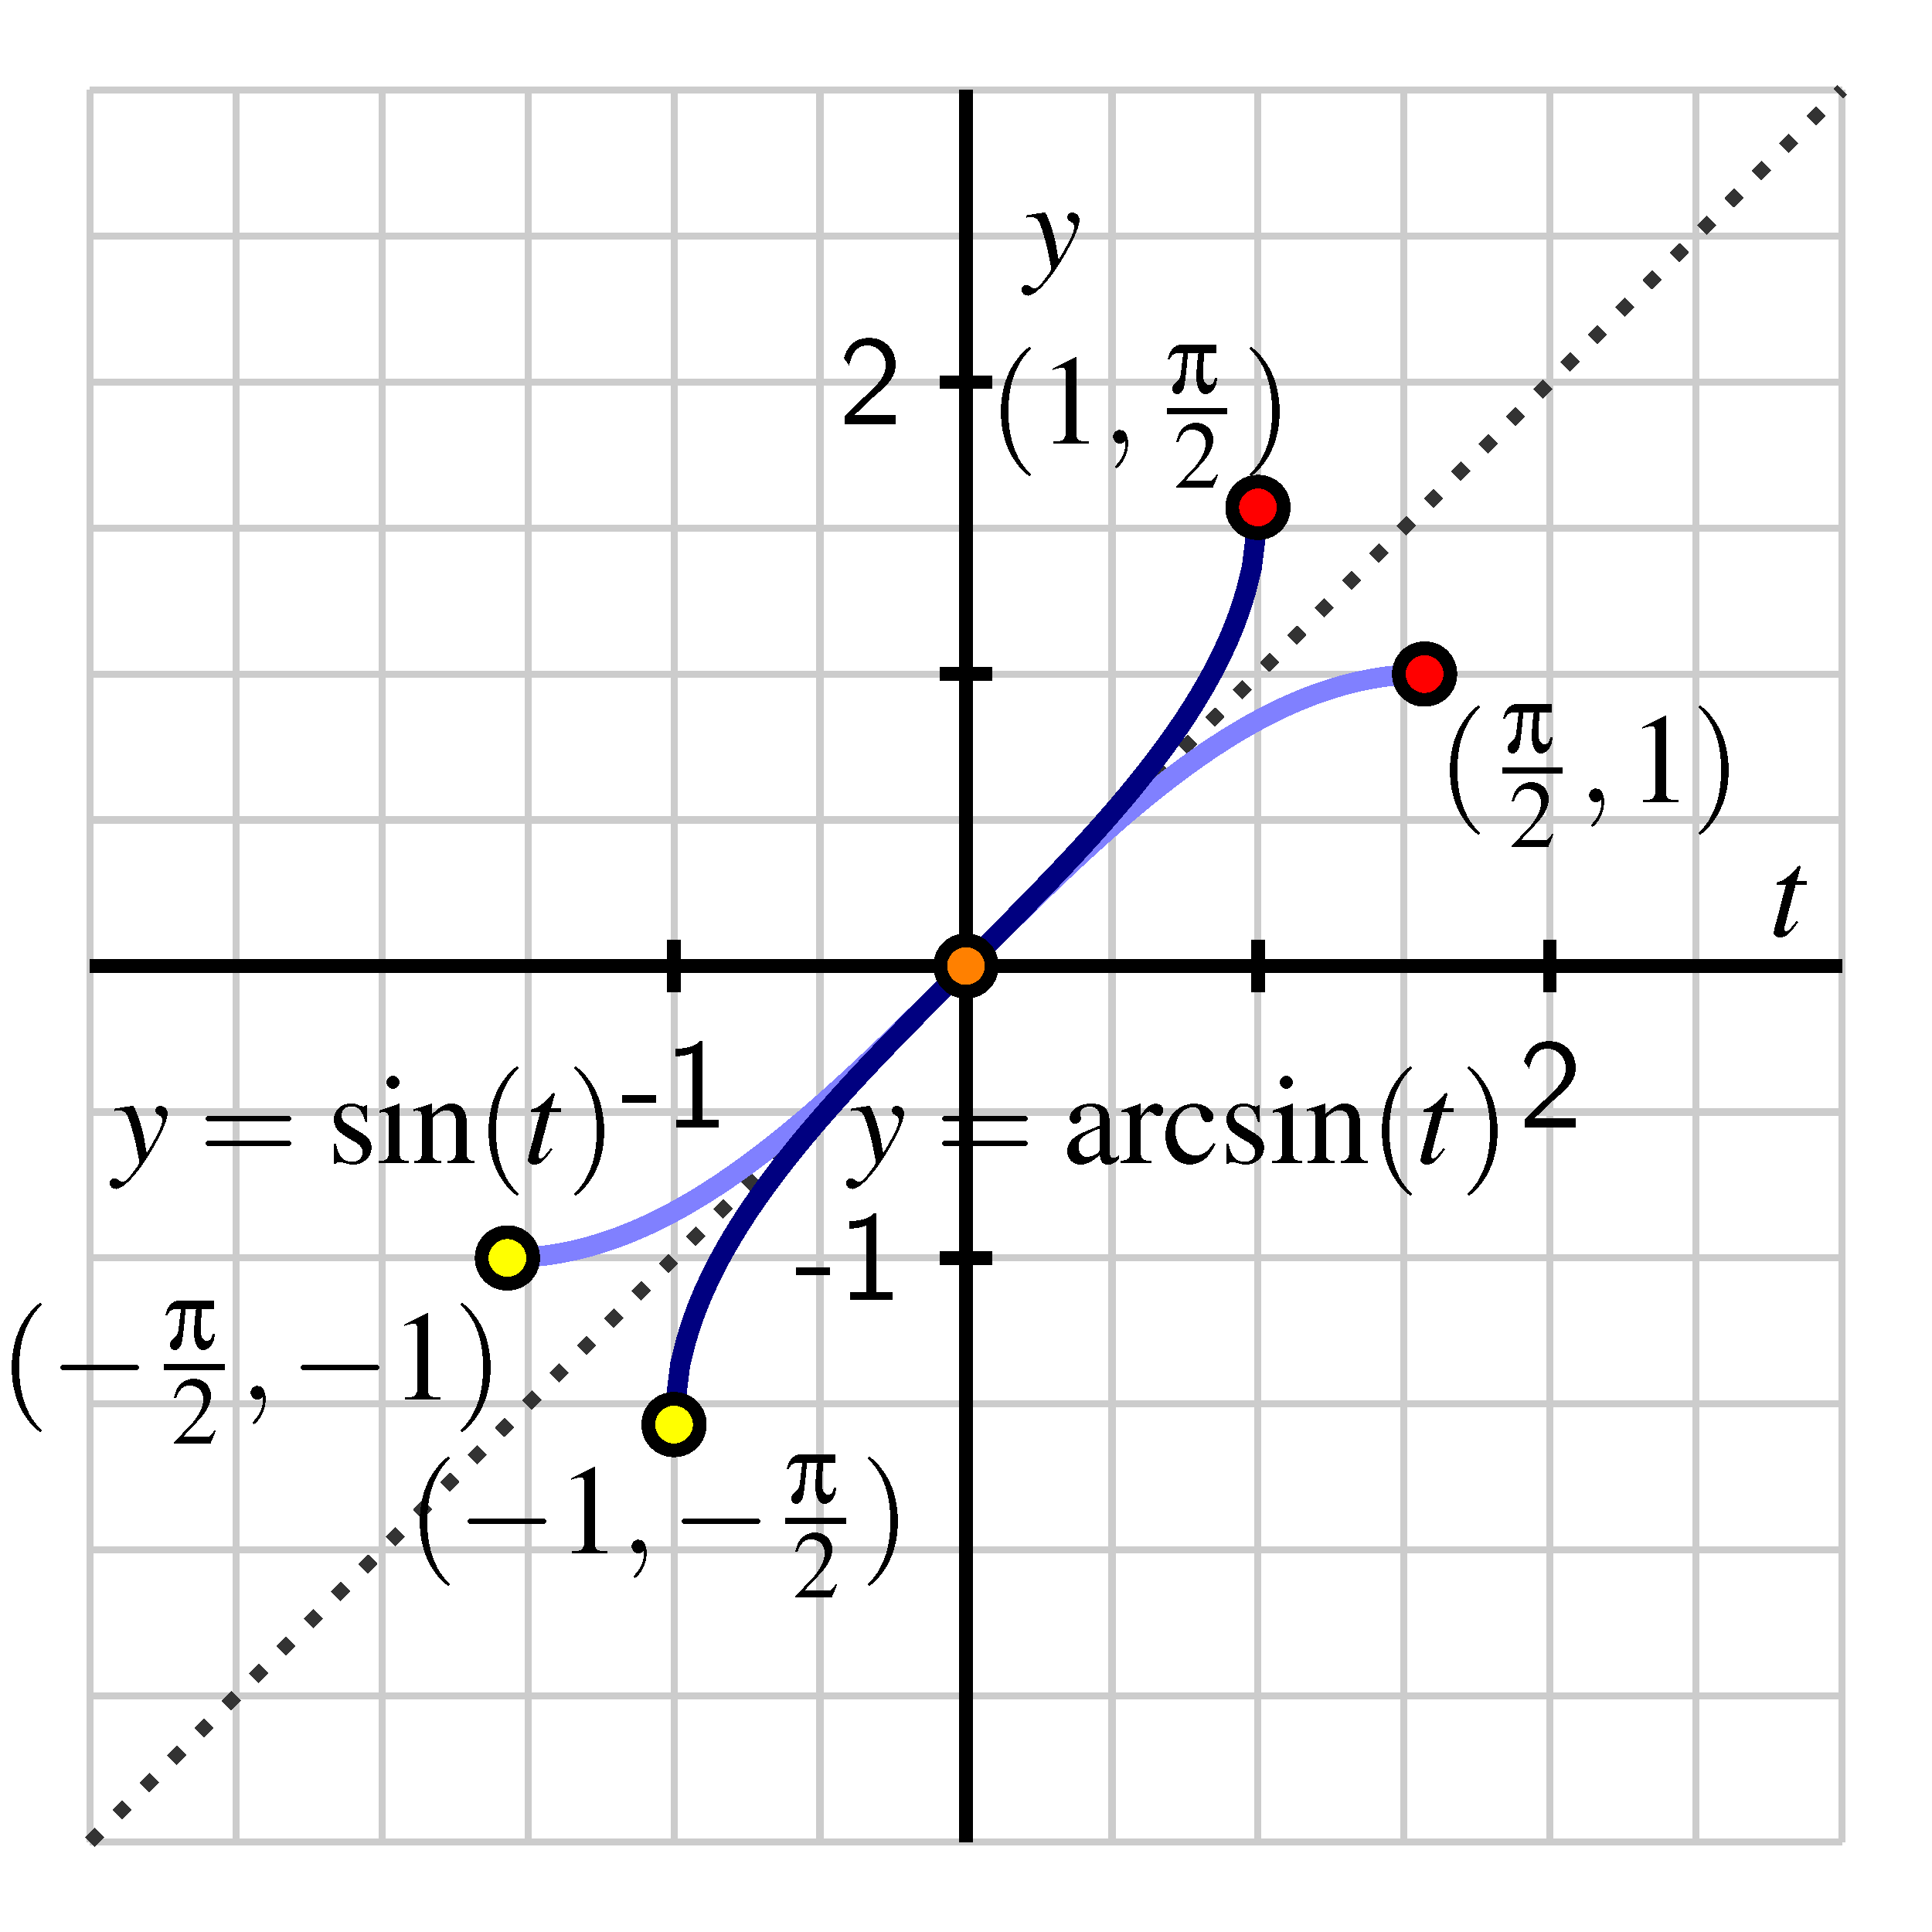
\includegraphics[width = .49\linewidth]{inverse-trig-arcsin-graph.png}
\end{image}
\par
The domain of $y = f^{-1}(t) = \arcsin(t)$ is $[-1,1]$ with corresponding range $[-\pi/2, \pi/2]$, and the arcsine function is always increasing.  These facts correspond to the domain and range of the restricted sine function and the fact that the restricted sine function is increasing on $[-\pi/2,\pi/2]$.%
\par
The domain of $y = h^{-1}(t) = \arctan(t)$ is the set of all real numbers with corresponding range $(-\pi/2, \pi/2)$, and the arctangent function is always increasing.  These facts correspond to the domain and range of the restricted tangent function and the fact that the restricted tangent function is increasing on $(-\pi/2,\pi/2)$.%
\begin{image}
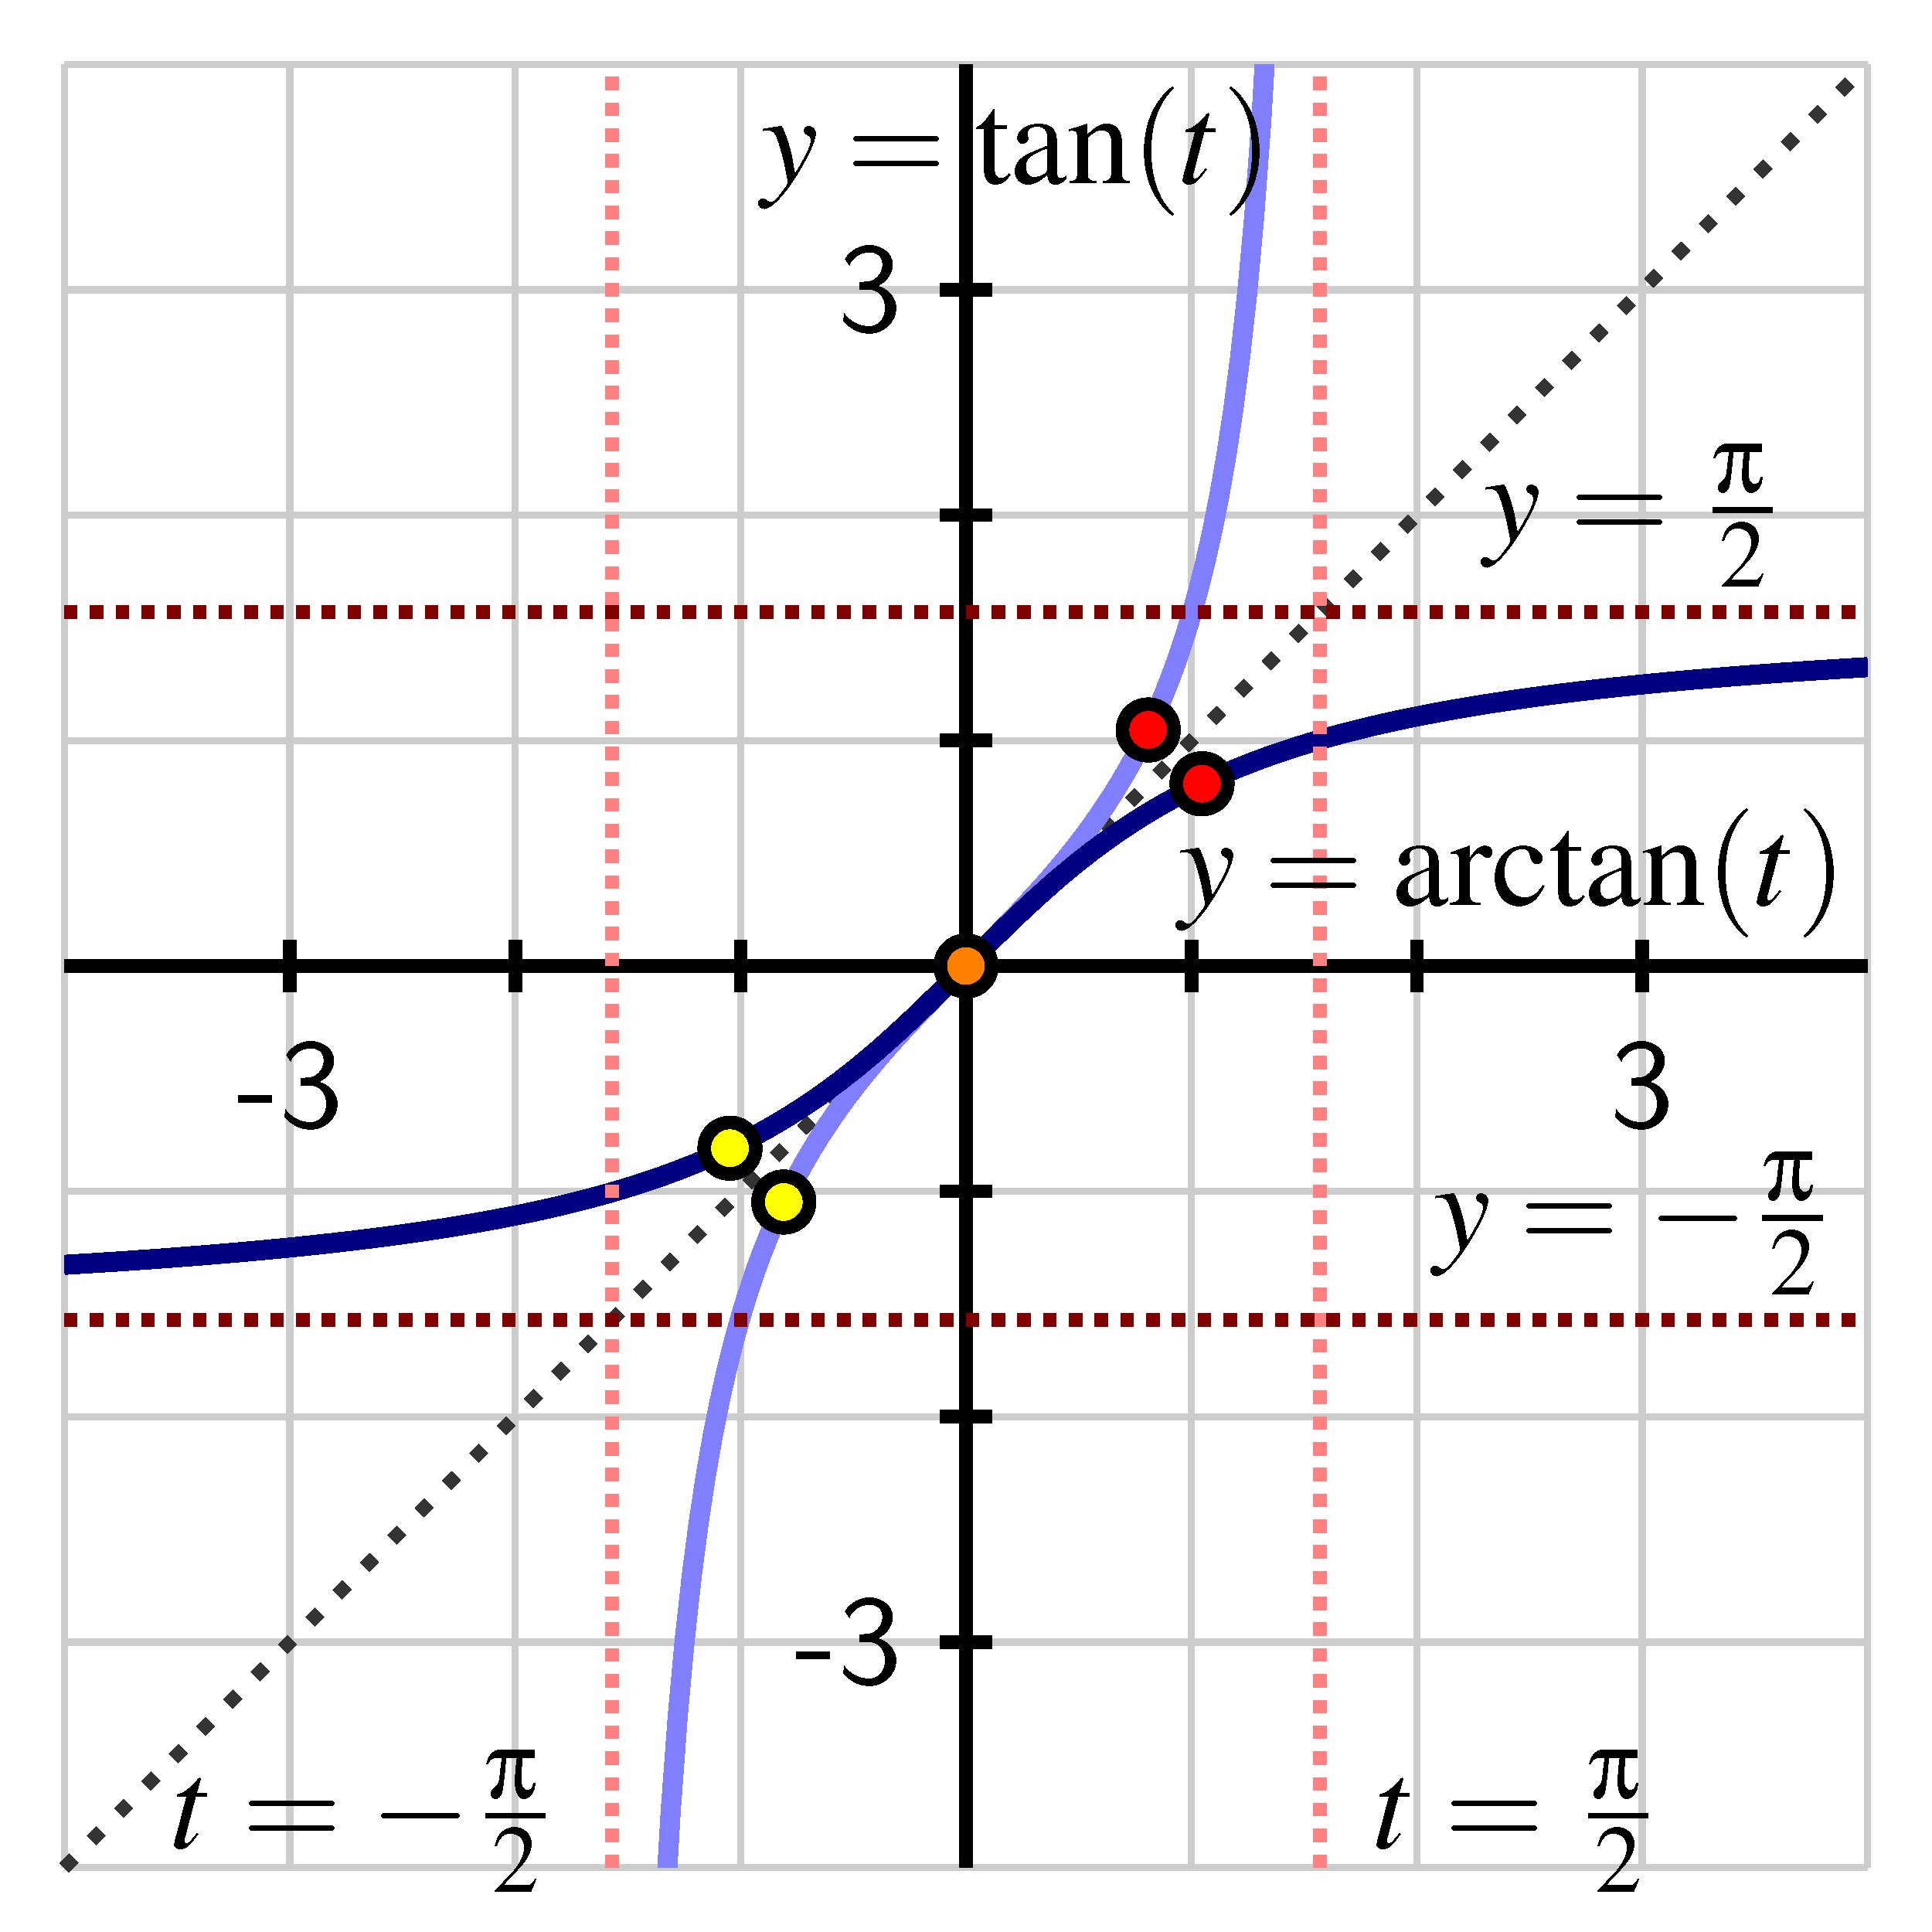
\includegraphics[width = .49\linewidth]{inverse-trig-arctan-graph.png}
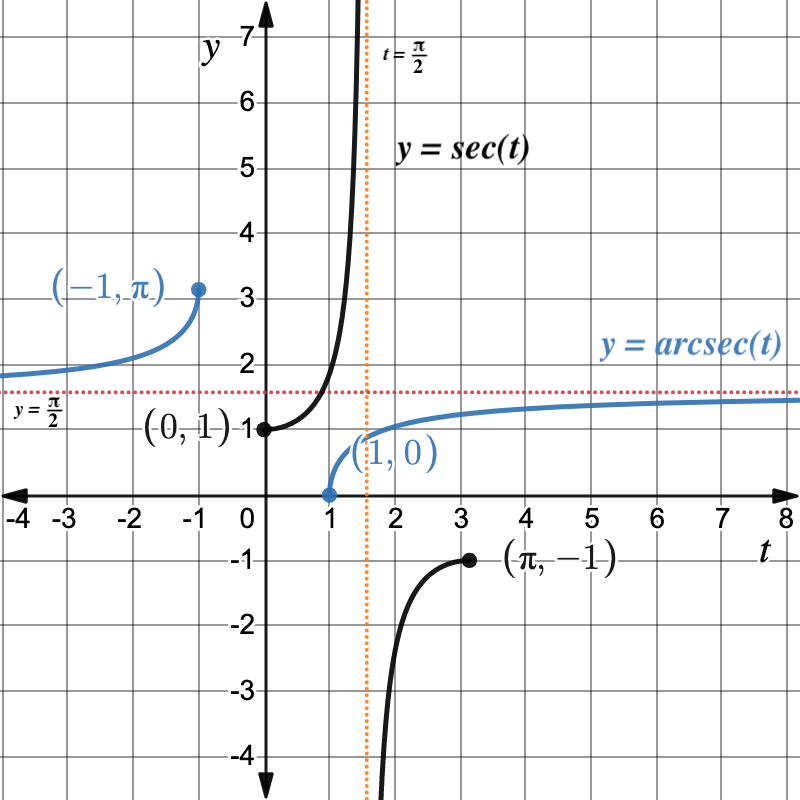
\includegraphics[width=.49\linewidth]{secArcsecGraphst.png}
\end{image}
\par
The domain of $y = k^{-1}(t) = \arcsec(t)$ is $(-\infty,-1] \cup [1,\infty)$,\footnote{We note that this may also be written as $\{x: |x| \geq 1\}$.} with corresponding range $[0,\pi/2) \cup (\pi/2, \pi]$. These facts correspond to the domain and range of the restricted secant function.
%
\end{itemize}
\end{summary}


\end{document}
